\documentclass[a4paper, 11pt, titlepage, twoside, openany]{book}
\usepackage{plain}
\usepackage{setspace}
% Layout
\usepackage[
  paperheight=29.7cm,
  paperwidth=21cm,
  outer=1.5cm,
  inner=2.5cm,
  top=2cm,
  bottom=2cm
]{geometry}
% Chapter
\usepackage{titlesec}
\singlespacing
\setcounter{secnumdepth}{3}
\setcounter{tocdepth}{3}
% Letter
\usepackage[utf8]{inputenc}
\usepackage{bold-extra}
% Language
\usepackage[english]{babel}
% Icons
\usepackage{fontawesome}
% PDF/A
\usepackage[a-1b]{pdfx}
% Image
\usepackage{graphicx}
\usepackage{wrapfig}
\usepackage{stackengine}
\usepackage{etoolbox}
\BeforeBeginEnvironment{wrapfigure}{\setlength{\intextsep}{0pt}}
% Hyperlink
\usepackage{xurl}
\usepackage[pdfa]{hyperref}
\hypersetup{breaklinks=true}
% Quote
\usepackage{csquotes}
\usepackage{epigraph}
\renewcommand{\mkbegdispquote}[2]{\itshape}
% Table
\usepackage{makecell}
\usepackage{xltabular}
\usepackage{hhline}
\usepackage{colortbl}
\usepackage{packages/slashbox}
\usepackage{caption}
\captionsetup[table]{position=bottom}
% List
\usepackage{enumitem}
% Color
\usepackage{xcolor}
\definecolor{gray}{RGB}{102,102,102}
\definecolor{green}{RGB}{0,153,0}
\definecolor{red}{RGB}{196,122,91}
\definecolor{bulmaBlue}{RGB}{32,156,238}
\definecolor{bulmaGreen}{RGB}{72,199,116}
\definecolor{bulmaRed}{RGB}{255,56,96}
\definecolor{shellGray}{RGB}{160,161,167}
\definecolor{shellBlue}{RGB}{64,120,242}
\definecolor{shellRed}{RGB}{228,86,73}
\definecolor{shellOrange}{RGB}{209,154,102}
\definecolor{shellGreen}{RGB}{80,161,79}
\definecolor{shellPurple}{RGB}{166,38,164}
\definecolor{iniOrange}{RGB}{209,154,102}
\definecolor{iniBlue}{RGB}{64,120,242}
\definecolor{iniGray}{RGB}{56,58,66}
\definecolor{yamlPurple}{RGB}{166,38,164}
\definecolor{yamlBlue}{RGB}{64,120,242}
\definecolor{yamlGreen}{RGB}{80,161,79}
\definecolor{yamlGray}{RGB}{160,161,167}
\definecolor{graphqlPurple}{RGB}{166,38,164}
\definecolor{graphqlGreen}{RGB}{80,161,79}
\definecolor{graphqlOrange}{RGB}{209,154,102}
\definecolor{graphqlGray}{RGB}{160,161,167}
\definecolor{graphqlBlue}{RGB}{64,120,242}
% Code
\usepackage{listings}
\usepackage{lstautogobble}
\usepackage{tikz}
\newcommand*{\circled}[1]{\tikz[baseline=(char.base)]{ \node[draw, shape=circle, inner sep=1pt, fill=black, text=white] (char) {#1};}}
\newcommand*{\icircled}[1]{\tikz[baseline=(char.base)]{ \node[draw, shape=circle, inner sep=1pt, line width=0.2pt] (char) {#1};}}


\lstset{ %
basicstyle=\ttfamily\footnotesize, %
columns=fullflexible, %
showstringspaces=false, %
numbers=left, %
numberstyle=\tiny\color{gray}, %
numbersep=5pt, %
backgroundcolor=\color{white}, %
showspaces=false, %
showtabs=false, %
frame=lines, %
rulecolor=\color{black}, %
tabsize=2, %
captionpos=b, %
breaklines=true, %
breakatwhitespace=false, %
keepspaces=true, %
title=\lstname, %
commentstyle=\color{green}\upshape, %
autogobble=true, %
keywordstyle=\bfseries %
}

\lstdefinelanguage{shell}
{ %
language=sh, %
alsoletter={-, +}, %
deletekeywords={set}, %
keywordstyle=\color{shellPurple}, %
morekeywords=[2]{set, rm, curl, sh, source, printf}, %
keywordstyle=[2]\color{shellRed}, %
morekeywords=[3]{-o, +o, -f}, %
keywordstyle=[3]\color{shellOrange}, %
keywordstyle=[4]\color{shellBlue}, %
stringstyle=\color{shellGreen}, %
commentstyle=\color{shellGray}\upshape %
}

\lstdefinelanguage{ini}
{ %
literate={{=}{{\textcolor{iniGray}{=}}}1}, %
keywordstyle=\color{iniBlue}, %
morecomment=[s][\color{iniOrange}]{[}{]}, %
morecomment=[l]{;} %
}

\lstdefinelanguage{yaml}
{ %
keywords={true, false, null}, %
keywordstyle=\color{yamlPurple}, %
keywordstyle=[2]\color{yamlBlue}, %
morestring=[b]', %
morestring=[b]", %
stringstyle=\color{yamlGreen}, %
comment=[l]{\#}, %
morecomment=[s]{/*}{*/}, %
commentstyle=\color{yamlGray}\upshape %
}

\lstdefinelanguage{graphql}
{ %
morekeywords={directive, on, enum, type}, %
keywordstyle=\color{graphqlPurple}, %
morekeywords=[2]{String, Int, Float, Boolean, Query, Mutation, Subscription}, %
keywordstyle=[2]\color{graphqlOrange}, %
morekeywords=[3]{FIELD, FIELD_DEFINITION, OBJECT}, %
keywordstyle=[3]\color{graphqlGreen}, %
keywordstyle=[4]\color{graphqlBlue}, %
morecomment=[l]{\#}, %
morecomment=[s]{"""}{"""}, %
commentstyle=\color{graphqlGray}\upshape %
}

% Document
\begin{document}
  % Cover
  \pagenumbering{gobble}
  \pagestyle{plain}
\thispagestyle{empty}


\begin{center}
  \begin{figure}[h!]
    \centering
    
\includegraphics[width=.6\textwidth]{images/logos/unitn.png}
  \end{figure}

  \vspace{2 cm}
  \LARGE{Department of Information Engineering and Computer Science\\}

  \vspace{1 cm}
  \Large{ Master's Degree in\\ Computer Science }

  \vspace{2 cm}
  \Large\textsc{Final Dissertation\\}
  \vspace{1 cm}
  \Huge\textsc{TODO\\}
  \vspace{0.5 em}
  \Large{\textit{TODO}}

  \vspace{2 cm}
  \begin{tabular*}{\textwidth}{c @{\extracolsep{\fill}} c}
    \Large{Supervisor}        & \Large{Student}         \\
    \Large{Lorenzo Angeli}    & \Large{Carlo Corradini} \\
    \Large{Co-Supervisor}     & \Large{223811}          \\
    \Large{Maurizio Marchese} & {}                      \\
  \end{tabular*}

  \vspace{2 cm}
  \Large{Academic year 2021/2022}
\end{center}
  \clearpage


  % Acknowledgements
  \thispagestyle{empty}


\begin{center}
  {\bf \Huge Acknowledgements}
\end{center}

\vspace{4cm}
\emph{TODO\ldots}
  \clearpage
  \pagestyle{plain}


  % Index
  \frontmatter
  \pagenumbering{Roman}
  \tableofcontents
  \clearpage


  % Start page numbering
  \mainmatter


  % Group to define space between chapters
  \begingroup
  % No page break between chapters
  % Override clear page commands
  % TODO Page break between chapters
  %\renewcommand{\cleardoublepage}{}
  %\renewcommand{\clearpage}{}
  % Override format of title chapter
  \titleformat{\chapter} {\normalfont\Huge\bfseries}{\thechapter}{1em}{} \titlespacing*{\chapter}{0pt}{0.59in}{0.02in}
  \titlespacing*{\section}{0pt}{0.20in}{0.02in} \titlespacing*{\subsection}{0pt}{0.10in}{0.02in}
  \titlespacing*{\subsubsection}{0pt}{0.05in}{0.02in}

  % Abstract
  \chapter*{Abstract}
\label{abtract}
\addcontentsline{toc}{chapter}{Abstract}


TODO


  % Chapters
  \chapter{Introduction}
\label{cha:introduction}

The purpose of this chapter is to provide an overview of the context, goals, and
core principles that serve as foundations for the overall cluster architecture,
both theoretical and implemented. \\ %
These so-called foundations are not restricted to this project and/or
environment, but can be considered as the minimum requirements and principles to
obtain a greener, energy and resource-aware software in general that is not only
for the present, but also, and must be, for the future, because we, as the overall
ICT community, have mostly ignored them in the past without giving them the
appropriate weight.

reCluster is heterogeneous because it is composed of numerous and diverse
components, ranging from computers to networking equipment, that have been
reutilized after decommissioning. The fundamental goal of reCluster is to establish
a cluster (hence the name) without reinventing the wheel, but rather to increase
reusability by transforming and adapting heterogeneous hardware and software
components designed for similar environments, enhancing the overall reduction of
both energy consumption and resources involved without compromising overall performance,
responsiveness, and ease of use.

\section{Context}
\label{sec:introduction_context}

Most existing systems rely entirely on large data centers, which are excessively
energy-hungry and do not provide any resource awareness owing to virtualization/abstraction
layers. Furthermore, the servers are maintained permanently powered on to significantly
minimize the time necessary for provisioning client instances while achieving virtually
100\% uptime\footnote{\url{https://aws.amazon.com/it/compute/sla}}\footnote{\url{https://azure.microsoft.com/support/legal/sla}}\footnote{\url{https://cloud.google.com/compute/sla}}.
\\ %
To achieve a greater degree of sustainability, the time necessary for provisioning
must be rebalanced, allowing servers to be completely powered off while
maintaining a similar level of uptime. It should be highlighted that this is ideal
for many applications that may be classified as non-critical, while critical
applications, such as emergency response and payment systems, require "five nines"
or 99.999\% or around five minutes and 15 seconds of downtime per year\footnote{\url{https://aws.amazon.com/blogs/publicsector/achieving-five-nines-cloud-justice-public-safety}}.

Radovanovi\'{c} et al., in \cite{carbon_aware_computing_datacenters}, describe
Google's Carbon-Intelligent Compute Management system, which actively reduces electricity-based
carbon footprint and power infrastructure costs by deferring temporally flexible
workloads. It uses a collection of analytical pipelines to acquire the next day's
carbon intensity projections, train day-ahead demand prediction models, and
apply risk-aware optimization to generate the next day's carbon-aware capacity
for all Google data centers. The system limits the resources available to temporally
flexible workloads on an hourly basis while preserving overall daily capacity,
allowing all such workloads to be completed within a day. \\ %
This type of computing solution only accounts for services and processes that
can be delayed, not those that must be continually active with an acceptable response
time; sending a critical email that is only delivered the following day is
unacceptable. It is only compatible with Google's data centers and does not provide
a more interoperable solution that is compatible with other data centers.
Moreover, the code is closed source, which means it does not adhere to the FLOSS
philosophy. Nevertheless, the notion of deferring non-real-time operations, employing
analysis and projections, to be rescheduled when the system is underutilized, improving
overall sustainability and lowering the costs, should be considered.

Enes et al., in \cite{power_budgeting_big_data_applications}, present a platform
that manages a power budget to limit the amount of energy spent by users,
applications, and individual container instances. The energy constraint is
accomplished by the platform's capability to monitor container energy
consumption and dynamically modify its CPU and memory resources via Vertical
Scaling as necessary (see section \ref{subsec:implementation_autoscaling_vertical_pod_autoscaler}).
\\ %
This approach is much more high-level and directly autoscale the resources
allocated to containers based on the power allocation among users and
applications, as opposed to a low-level approach that involves physically terminating/bootstrapping
the server (used by reCluster). Moreover, the energy is viewed as a precious resource
that can be split and shared, improving the container system's overall awareness
of its resources. Nevertheless, it needs to be combined with additional
approaches to achieve high and low levels of energy awareness and reduction.

Paya and Marinescu, in \cite{energy_aware_load_balancing}, presented an energy-aware
operation model for load balancing and application scaling on a cloud, outlining
an energy-optimal operation regime and aiming to increase the number of servers employed
in this regime. Servers that are idle or only barely loaded are put into one of
the sleep modes to conserve energy. Therefore, the following could be employed
to reformulate the conventional idea of load balancing in a large-scale system: \textit{"Distribute
evenly the workload to the smallest set of servers operating at optimal or near-optimal
energy levels, while observing the Service Level Agreement (SLA) between the Cloud
Service Provider (CSP) and a cloud user. An optimal energy level is one when the
performance per Watt of power is maximized"}. \\ %
To reduce energy waste, this approach can be applied to an external load balancer
employed in the architecture. Even more, energy can be saved by completely turning
off mostly inactive or lightly-loaded servers rather than switching them into sleep
mode. This new type of load balancer can also be interfaced with the Cluster
Autoscaler and Server to better understand the overall cluster state, both in terms
of active/inactive nodes and also of overall power consumption, to obtain more
fine-grained information and therefore increase the overall efficiency.

All of the above strategies attempt to minimize energy consumption in various
contexts: non-real-time services, containerization, and load balancing. Yet, none
of them address, or only partially address, the core cause of the highest energy
usage in a cluster architecture, which is the server themselves. To establish a more
sustainable and resource-aware cluster, the servers must be considered and
therefore autoscaled by physically bootstrapping or terminating them; since a powered-off
machine consumes (nearly) zero energy. \\ %
Nonetheless, the prior techniques should, and must, be extended into future
versions of reCluster to achieve even higher levels of energy reduction while
satisfying the SLA. \\ %
More than ever, a more sustainable cluster architecture is required.

\section{Goals}
\label{sec:introduction_goals}

A cluster is composed of several components, including hardware and software,
that operate together as a single entity to accomplish one homogeneous goal, or multiple
and different goals. The hardware components, which are typically computers of different
kinds ranging from desktop computers to single board computers, are connected in
a single network: the cluster network, by additional hardware components
particularly designed for communication. Because multiple applications can achieve
the same result, are constantly evolving with newer features and capabilities, and
can be employed or not depending on the (current) needs and requirements, the
software components can vary and are as heterogeneous as the hardware, if not more.
Between hardware and software, two major distinctions complement one another.
The first distinction is that hardware, particularly reconditioned hardware, is
limited in its ability to be modified and transformed, whereas software is essentially
limitless in this regard and may achieve the same goal using multiple technologies
and/or languages. The second distinction is that there is no difference between
the various hardware components in terms of whether they are used for cluster
operations or user operations. Instead, software components can be divided into
low-level ones that are used to keep the overall cluster operational and high-level
ones that are used by the users for their specific services. In this context,
software in all of its aspects must be used to compensate for the shortcomings
of the hardware since it can be customized to fill the gaps where the hardware
lacks. \\ %
Most used hardware components may be reconditioned by reusing decommissioned
components from consumers and organizations due to upgrades. Because newer components
are often more performant and energy-efficient than older ones, the hardware is
directly and automatically managed by the various cluster-related software
deployed. \\ %
The cluster must be as simple as possible, with human interaction minimized to nearly
zero, and automatic solutions preferred. The most essential automated solution that
must be implemented in a cluster is autoscaling, both upscaling and downscaling.
In upscaling, the cluster automatically bootstraps an inactive hardware
component. Whereas in downscaling, the cluster automatically terminates an
active hardware component. Selecting which component(s) to autoscale can follow
multiple criteria, such as choosing nodes that are more power efficient or performant,
or even a combination of the two. The latter is an excellent illustration of the
combination of hardware and software that needs to be present in the cluster. \\ %
The cluster should be used in a wide range of environments and use-case scenarios,
from a modest and local deployment at home to a large and remote deployment
comparable to that found in a data center. Given that the various software manages
them automatically using the autoscaling technique, there should be no limit to
the number of involved computers. \\ %
If there is no need to operate the cluster for specific periods and it is
therefore considered worthless, it can be completely shut down, with the benefit
of reducing its overall power consumption to zero. When it is necessary again,
it is reactivated. Although the latter may create some performance and/or responsiveness
issues, because no physical machines are managing any service, it is far preferable
to an always-on technique. The latter impacts can be mitigated if the
organization can calculate different models and/or employs a single board
computer as the always-on hardware component thanks to its overall extremely low
power consumption. As stated previously, the context is dynamic, and hence the latter
is dependent on the organization in charge of the cluster.

As a result, the cluster should appear less heterogeneous and more like a
homogenous, and mostly automated entity.

\section{Principles}
\label{sec:introduction_principles}

This section is dedicated to illustrating some of the fundamental principles
around which the overall design is based. These principles should be seen as the
foundations for a more sustainable, resource-aware, free and open-source, and
energy-efficient architecture that may be utilized not only in this specific
context, but in all aspects of ICT. \\ %
It should be highlighted that these principles should not be regarded as negative
to overall performance and responsiveness, but rather as equally important. Performance
and responsiveness currently constitute the sole and most significant characteristics
to consider when examining software, but in the future, it should be necessary,
almost mandatory, to include, maybe gradually but starting to consider them as
parameters for comparisons and essential aspects of a program. \\ %
The applicability of these principles is determined by the organization's
requirements. Yet, some of these principles should be investigated and
implemented in the future for greener and more resource-aware software. \\ %
The proposed list can undoubtedly be improved upon and/or expanded with
additional, and possibly more strict, principles. Shifting the computing industry
toward a more sustainable future should be possible, if not essential.

\subsection{Sustainability}
\label{subsec:introduction_principles_sustainability}

\begin{wrapfigure}
  {l}{.2\textwidth} %
  \centering
  \def\stackalignment{l}\stackunder{ 
\includegraphics[width=\linewidth]{images/logos/sdgs.png} } %
  {\scriptsize \parbox[t]{\linewidth}{ Source: \url{https://www.un.org/sustainabledevelopment/news/communications-material}} }
\end{wrapfigure}

The United Nations (UN) has established 17 Sustainable Development Goals\footnote{\url{https://sdgs.un.org}}
(SDGs). The SDGs address climate change and strive to preserve the oceans and forests,
while also addressing poverty and other deprivations via initiatives that
improve health and education, reduce inequality, and stimulate economic growth. \\ %
Clearly, in an ICT context, several of these Goals may appear to be out-of-context,
unreachable/unfeasible, or not directly related. However, the majority of them, including
those that are not directly related to an ICT context, must be considered when
developing new software applications and architectures; given that a minor improvement
in a single SDG can benefit all other SDGs. There is no need to change or
entirely disrupt a project's primary goal, but rather to integrate the relevance
of these long-term goals into the development process. If an ICT initiative
improves or enhances one or more SDGs, it will undoubtedly benefit not only other
direct and associated SDGs, but practically every other SDG as well. \\ %
A large end goal is nearly always comprised of a plethora of many smaller
improvements/objectives that, when considered separately, may appear to be
irrelevant, but when placed together form a sustainable chain of progress.

\subsection{Acknowledging Planetary Limits}
\label{subsec:introduction_principles_acknowledging_planetary_limits}

\begin{wrapfigure}
  {l}{.2\textwidth} %
  \centering
  \def\stackalignment{l}\stackunder{ 
\includegraphics[width=\linewidth]{images/introduction/limits.png} } %
  {\scriptsize \parbox[t]{\linewidth}{ Icon made by \href{https://www.flaticon.com/authors/freepik}{Freepik} from \href{http://www.flaticon.com}{www.flaticon.com} }}
\end{wrapfigure}

When available resources are limited, it is essential to preserve them and
reduce their overall consumption as much as possible. It is important to note that
the term resources in this context is more generalized and does not designate any
specific resource type, but they may be regarded as a distinct entity that
groups them. \\ %
Rethink and change the availability of resources, and investigate a more realistic
and conservative approach, referred to in \cite{computing_within_limits} as
computing within limits or simply LIMITS. LIMITS incorporates three major topics:
present and near-future ecological, material, and energy constraints; new forms of
computing that may assist promote well-being while living within these limits;
and the influence of these limits on the area of computing. Not only is the concept
of LIMITS confined within a computing environment, but it also aims to integrate
other, and sometimes uncorrelated, heterogeneous areas. Moreover, because
resources are not exclusively available to individuals, there is a need to think
about and focus on collectives and larger contexts engaging in stronger connections
to sustainable activities in disciplines other than computing. The term resource(s)
should be considered not just to describe actual elements, but also to encompass
socioeconomic, more intangible, factors that may be enhanced by diverse
techniques pursued by the computing community, such as promoting development rather
than economic growth. \\ %
As stated in \cite{ed_tech}, the incorrect underlying assumptions of endless, infinite,
and replicable technological resources must be reconsidered. These assumptions are
just unsuitable for a more constrained and sustainable future. To re-imagine how
digital technologies may be developed and implemented in these new and limited
computing architectures, new concepts of radically leaner and ecologically conscious
techniques are necessary. \\ %
Another element of the architecture's involved resources is the relationship between
the software and the hardware. Because of the current amount of processing power,
some software has ridiculously high hardware requirements for even the most simple
operations. Better and more performant programming languages and algorithms need
to be employed to rethink, modify, and/or improve software resource requirements.
A different technique is necessary with the adoption of a more permacultural approach,
which is referred to as permacomputing in a computing environment. Permacomputing,
as depicted in \cite{permacomputing}, is both a concept and a community of practice
centered on issues of resilience and regenerative in digital technology,
transforming problems into solutions, competition into cooperation, and waste
into resources. \\ %
Transform what appears to be a disadvantage, a difficulty, or even a waste into
a rich and valuable resource.

\subsection{Hardware Reusability}
\label{subsec:introduction_principles_hardware_reusability}

\begin{wrapfigure}
  {l}{.2\textwidth} %
  \centering
  \def\stackalignment{l}\stackunder{ 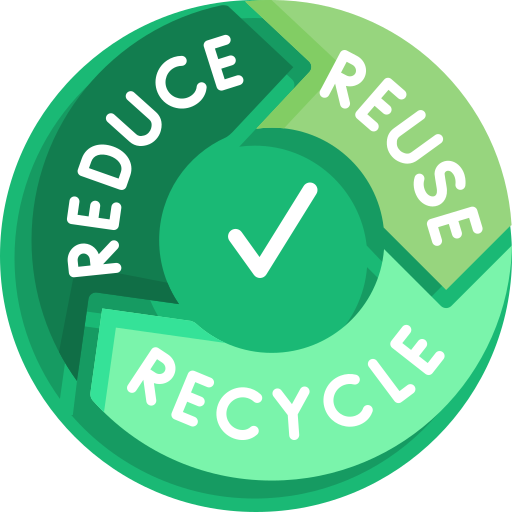
\includegraphics[width=\linewidth]{images/introduction/recycle.png} } %
  {\scriptsize \parbox[t]{\linewidth}{ Icon made by \href{https://www.flaticon.com/authors/freepik}{Freepik} from \href{http://www.flaticon.com}{www.flaticon.com} }}
\end{wrapfigure}

Use reusability and repairability approaches to reduce resource waste as much as
possible. \\ %
The majority of unused hardware is perfectly capable of fulfilling the majority
of tasks and operations in sustainable architecture, such as hosting a website or
a cache server, without any particular difficulty. Unused hardware is frequently
created by an upgrade to a newer and more recent version or by (major) scheduled
decommissioning. \\ %
Typical electronic devices with even a single faulty hardware component are discarded
and promptly replaced with newer hardware, even if the remaining components are
healthy and completely functional. The expenses and work required for a repair vary
depending on the device, but most of the time the repair may be performed
quickly and cheaply by replacing the faulty component with a new one. Furthermore,
and this is especially true for desktop computers, if two devices are compatible
and one has some broken components that the other does not, the healthy
components can be combined to re-create a single but healthy and usable device
with the benefit of drastically reducing the overall amount of resource waste. \\ %
The latter two approaches not only recycle abandoned technology but also reduce
the overall quantity of electronic waste (e-waste) that they can generate. Consequently,
the energy gap between overall utilization energy and production energy, formerly
expressed as embodied energy, can be narrowed or even attained and exceeded. \\ %
Yet, the ease and feasibility of a device's repairability is entirely dependent on
its manufacturer. Moreover, there are cases where the devices have a planned obsolescence
after which some of the components will probably break and the cost or effort required
for a repair is unfeasible, and it is far easier to buy a new one while
discarding the old and broken one, causing additional (e-)waste. It is difficult
to avoid the latter, and almost certainly additional issues, induced by the
manufacturer. Yet, in recent years, there have been an increasing number of consumer
activities aimed at reducing or eliminating the behaviors perpetuated by these manufacturers.
The Right To Repair\footnote{\url{https://www.repair.org}}\footnote{\url{https://repair.eu}}
movement is the most well-known, to advocate for repair-friendly policies,
regulations, statutes, and standards. Another approach is to provide a repairability
index, such as the French repair index\footnote{\url{https://www.ecologie.gouv.fr/indice-reparabilite}},
for the products so that potential customers may know and understand how easy it
is to repair the corresponding device before purchase. It should be noted that
not all manufacturers are opposed to repairability, and there are certain,
albeit small, manufacturers, such as Framework\footnote{\url{https://frame.work}},
that have repairability as one of their core missions, building longevity
products and improving the overall availability of spare parts and ease of
upgrade, customization, and repairability. The objective/hope is that more manufacturers
will begin to design, produce, and distribute more sustainable products. \\ %
Instead of planned obsolescence, consider planned longevity.

\subsection{Energy Reduction}
\label{subsec:introduction_principles_energy_reduction}

\begin{wrapfigure}
  {l}{.2\textwidth} %
  \centering
  \def\stackalignment{l}\stackunder{ 
\includegraphics[width=\linewidth]{images/introduction/energy.png} } %
  {\scriptsize \parbox[t]{\linewidth}{ Icon made by \href{https://www.flaticon.com/authors/freepik}{Freepik} from \href{http://www.flaticon.com}{www.flaticon.com} }}
\end{wrapfigure}

The architectures and software should strive to reduce their total energy
footprint as much as possible while providing similar, if not identical,
outcomes. Concerning the preceding point, this is only possible if the
organization has complete control over all aspects of the architecture, since the
union of software and hardware is the only conceivable and feasible strategy to establishing
a more sustainable and energy-aware architecture. \\ %
Energy is one of the most significant factors in achieving sustainable architecture.
Because energy is closely related to carbon emissions, there is a need for low-carbon
and sustainable computing with a path towards zero-carbon computing, as stated
in \cite{frugal_computing}, because current computing emissions account for about
2\% of global emissions and are expected to rise dramatically in the upcoming
years. This rate of expansion is unsustainable and as a community, we must begin
to regard computational resources as finite and valuable, to be used only as essential
and as effectively as possible. The latter is known as frugal computing, and it strives
to get the same outcomes while using less energy by being more frugal with the available
computing resources. In the current context, for example, if a system/computer
in a cluster is not needed or is underutilized, it is a waste of both energy and
resources. It must be terminated and, if any services are deployed on it,
migrated to another active system to avoid service interruptions, increasing its
utilization and lowering the architecture's total power consumption while maintaining
the same level of Quality of Service (QoS). Humans are unable to perform these
operations since there is the need to continuously monitor and check the overall
status of the entire architecture. The core principles of energy reduction must be
developed into automatic systems that could be easily extended to existing applications
and tools which are focused solely on overall system performance and responsiveness.
The system should be as efficient as possible, employing only those components that
are strictly necessary, avoiding bootstrapping unneeded machines and terminating
those that are unnecessary, and avoiding the paradigm of an always-on architecture
that wastes energy and resources. \\ %
Another factor to consider is the embodied energy of each hardware system.
Embodied energy is the energy necessary to build all of the electronic
components (both network and especially consumer appliances). It emerges that the
energy used to manufacture electronic components is significantly higher, and in
many cases dominant, than the energy needed throughout their whole operation\cite{monster_footprint}.
This means that practically every hardware component is underutilized in terms of
the energy required for manufacturing it. As a result, there is a need to correct
this imbalance by attempting to reach at least the same amount of energy. It
should be noted that the latter does not want to employ the hardware
unconsciously, but rather with better and more conscious principles and logic that
not only tries to reduce the overall "live" energy consumption, but also tries
to equal, if not even surpass, the embodied energy of each electronic device
that is employed in the architecture. \\ %
Previously, the term carbon emission/footprint was used concerning energy consumption.
Yet, it is necessary to accurately define how the overall energy of the architecture
is estimated, as well as the fundamental principles on which the calculation is
based. This is not as simple as it appears. \cite{world_wide_web_carbon} reveal
that quantifying the carbon footprint has produced contradictory results, implying
the need for different and alternative approaches that delineate the specific relationships
between elements - geographic, technical, and social - within the broader information
and communication technologies infrastructure. The common method of assessing
the energy impacts is the kilowatt hours of electricity and gigabytes of data
through a network, expressed as the functional unit \texttt{KWh/GB}. The \texttt{KWh/subscriber}
metric, which divides the larger energy draw inside a study's system boundary by
the number of subscribers within the network, can better represent worldwide
patterns in network access expansion over time. Rather than calculating \texttt{KWh/GB}
or \texttt{KWh/subscriber}, a relational approach would assess the carbon, water,
and land footprints of powering the whole architecture in specific regions of
the world, highlighting the significant disparities between the various locations.
Network shapes, rather than scales, provide new possibilities for assessing the
existing and future Internet\cite{world_wide_web_carbon}.

\subsection{Insourcing}
\label{subsec:introduction_principles_insourcing}

\begin{wrapfigure}
  {l}{.2\textwidth} %
  \centering
  \def\stackalignment{l}\stackunder{ 
\includegraphics[width=\linewidth]{images/introduction/insourcing.png} } %
  {\scriptsize \parbox[t]{\linewidth}{ Icon made by \href{https://www.flaticon.com/authors/kerismaker}{kerismaker} from \href{http://www.flaticon.com}{www.flaticon.com} }}
\end{wrapfigure}

Invert the trend of constantly outsourcing applications to third-party cloud providers;
we might express this with a neologism: "Insourcing". \\ %
While there are undeniable benefits to outsourcing in terms of convenience and better
pricing, it erodes institutional and human independence by centralizing a single
point of failure and delegating relevant choices regarding privacy, data ownership,
and environmental impact on these external actors\cite{conceptualising_resource_aware}.
\\ %
There is a need to obtain, direct control over the whole software stack, beginning
with the hardware infrastructure and progressing through the application's development
and final release. At first look, reversing the ICT outsourcing trend may appear
to be impracticable, unneeded, and comparable to an old and mostly outdated approach.
Nonetheless, overall technology, tools, and usability have significantly improved
in recent years. Most importantly, there has been a shift in the software community
toward standardization and interoperability across heterogeneous systems, which
has not only made deploying software locally and with an in-house infrastructure
trivial, but has also aided in abstracting away from the final user common and not-so-trivial
problems, such as handling and coordinating multiple connections across
different hardware and software components/layers. \\ %
As discussed in \cite{precarious_infrastructure} current infrastructures and
approaches to climate change are mitigation-oriented, aiming only to support or investigate
social changes that reduce the material causes of the more pernicious facets of global
change, with the implicit assumption that these infrastructures will persist as
the risks of current unsustainable practices become urgent threats to well-being
and survival. Instead, new architectures, and possibly old ones through refactoring
and rethinking the overall design, must take and address new approaches, denoted
as post-apocalyptic computing, to address the many, dramatic, and complex
phenomena associated with global change, allowing to prepare for nonlinear changes.
If the organization has direct control over almost every aspect of the
architecture, the latter can be accomplished with almost negligible effort,
whereas if everything is outsourced to an external entity, the organization has only
a limited amount of control over the possible future outcomes that can arise from
unpredictable changes that will occur sooner or later. As a result, avoid remote
and generally unknown architectures of third-party organizations that only raise
the fragile state on which the application is deployed, establishing an inherent
single point of failure that not only can be an issue for the present but, more significantly,
for the future. \\ %
Another significant aspect of current architectures and approaches is that most
operations are performed remotely and outsourced to external organizations, even
though the participating entities are mostly close together, resulting in extra
workload and networking equipment, which translates to an increased amount of overall
power consumption. In this regard, the usage of external videoconferencing applications
that enable remote entities to connect is a significant example. When two close
entities, that can be even in the same building, seek to establish a
teleconference, their data is routed to remote videoconferencing servers.
Instead of depending on an external and remote service, it is possible to set up
a local videoconferencing service in the local (insourced) architecture,
employing open-source software and improving overall security and privacy. The distance
between the entities and the local server instance may be drastically reduced,
decreasing latency and lowering total power consumption for the videoconference,
as theorized in \cite{comparison_energy_carbon_time_videoconferencing},
resulting in better outcomes and more sustainable service. \\ %
Lastly, insourcing enables better fine-grained and conscious control over the whole
application's data and everything that comes with it, such as privacy and
security, because it is known where and how it is stored, distributed, and protected.
Even though these later elements are not the primary focus of this document, they
should not be ignored or underestimated because they are essential for almost every
software application. Furthermore, various initiatives in recent years have attempted
to improve data protection for individuals and organizations, including the well-known
General Data Protection Regulation\footnote{\url{https://gdpr.eu}} (GDPR)
drafted and passed by the European Union (EU). \\ %
As a result, returning to an insourcing approach and having direct control over almost
every aspect of the architecture and software stack is not only feasible and almost
trivial nowadays, but also necessary for establishing a better and more
sustainable future for everybody, not just the individual.

\subsection{Interoperability}
\label{subsec:introduction_principles_interoperability}

\begin{wrapfigure}
  {l}{.2\textwidth} %
  \centering
  \def\stackalignment{l}\stackunder{ 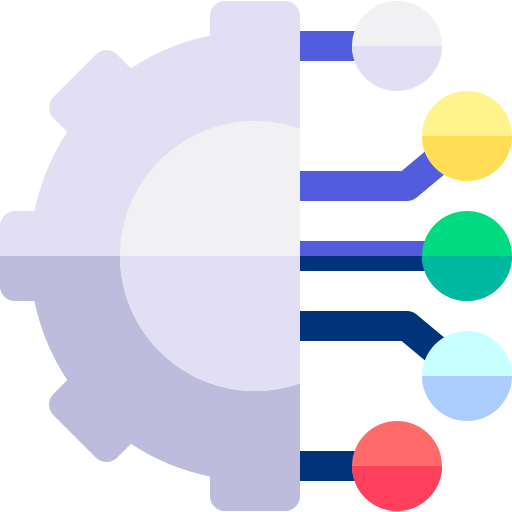
\includegraphics[width=\linewidth]{images/introduction/interoperability.png} } %
  {\scriptsize \parbox[t]{\linewidth}{ Icon made by \href{https://www.flaticon.com/authors/freepik}{Freepik} from \href{http://www.flaticon.com}{www.flaticon.com} }}
\end{wrapfigure}

Interoperability and standardization of hardware and software must be at the core
of a more sustainable architecture. Most, if not all, of the components, employed
in the design must agree on common interfaces to prevent the need for hardware adapters
and software translation layers, which not only increase resource waste and
energy consumption but also decrease overall system performance. \\ %
When all of the applications employed by the architecture agree on or adapt to a
common set of interfaces, achieving software interoperability is virtually straightforward.
Upgrading previously incompatible software is feasible, albeit depending on the complexity
of the program, refactoring may be required. Fortunately, most software programs
and, more broadly, the computing environment depends on standards that are
equivalent in practically every part of the world. Consider the Internet itself,
which is built on standards and interoperability between all sorts of
heterogeneous components. \\ %
On the other hand, implementing hardware interoperability and standardization is
considerably more challenging than software since it is heavily dependent on design
decisions made by the manufacturer throughout the development phases. As a
result, there is a need to persuade, mostly through legislation, the many manufacturers
that are reluctant to adapt and do not meet or do not want to establish a set of
standards that improve interoperability on their devices. A perfect example of
the latter is the European Parliament's approval of a law, following an impact assessment
study\footnote{\url{https://data.europa.eu/doi/10.2873/528465}}, that mandates
by the end of 2024 a common, standardized, and interoperable charger for all
mobile devices sold in the EU internal market\footnote{\url{https://www.europarl.europa.eu/news/en/press-room/20220930IPR41928/long-awaited-common-charger-for-mobile-devices-will-be-a-reality-in-2024}}.
The latter has been highly awaited, and it may be regarded as a first step
toward a much broader trend of standardization and interoperability that can
establish the foundation for a more sustainable future. \\ %
Furthermore, they can significantly reduce the effort required while also increasing
the ease of establishing an insourcing architecture. Various organizations can
exploit a uniform and de-facto standard that enables high-level interoperability
between heterogeneous architectures, accelerating the process of migrating various
services and deployments from remote to local architectures. \\ %
Lastly, having an interoperable architecture, combining software and hardware,
eliminates the so-called technology vendor lock-in effect, in which a customer is
dependent on a single manufacturer. Because the entire architecture might be
composed of reconditioned/refurbished hardware and thus is intrinsically
heterogeneous, the vendor lock-in effect cannot be tolerated.

\subsection{Free/Libre And Open Source Software}
\label{subsec:introduction_principles_free_libre_and_open_source_software}

\begin{wrapfigure}
  {l}{.2\textwidth} %
  \centering
  \def\stackalignment{l}\stackunder{ 
\includegraphics[width=\linewidth]{images/logos/open_source.png} } %
  {\scriptsize \parbox[t]{\linewidth}{ Source: \url{https://opensource.org/logo-usage-guidelines}} }
\end{wrapfigure}

The software developed and employed in the architecture must be Free/Libre and Open
Source in all aspects. If a software application is incompatible with the latter,
an alternative must be identified or developed. \\ %
Following the GNU Project's philosophy\footnote{\url{https://www.gnu.org/philosophy}}:
\textit{Free Software means that users have the four essential freedoms: (0) to run
the program, (1) to study and change the program in source code form, (2) to redistribute
exact copies, and (3) to distribute modified versions.} \\ %
This principle's fundamental is presented as Free/Libre and Open Source Software\footnote{\url{https://www.gnu.org/philosophy/floss-and-foss.html}}
(FLOSS). \\ %
Being FLOSS-compatible has also the significant advantage of allowing external programmers
to contribute to the software, consequently improving overall quality and
providing for more performant and efficient logic and algorithms.

\subsection{Dependencies Reduction}
\label{subsec:introduction_principles_dependencies_reduction}

\begin{wrapfigure}
  {l}{.2\textwidth} %
  \centering
  \def\stackalignment{l}\stackunder{ 
\includegraphics[width=\linewidth]{images/introduction/packages.png} } %
  {\scriptsize \parbox[t]{\linewidth}{ Icon made by \href{https://www.flaticon.com/authors/freepik}{Freepik} from \href{http://www.flaticon.com}{www.flaticon.com} }}
\end{wrapfigure}

For decades, as stated in \cite{software_dependency_problem}, discussion about
software reuse was more widespread than real software reuse. Nowadays, the
situation is reversed, with developers reusing software produced by others regularly
in the form of software dependencies, and the situation is largely unexamined. Software
dependencies pose substantial risks that are all too often ignored. The
transition to easy, fine-grained software reuse has occurred so quickly that there
is little knowledge of the best practices for identifying and using dependencies
effectively, or even determining when they are appropriate and when they are not.
Installing a package as a dependency outsources the effort of developing that code
--- designing, writing, testing, debugging, and maintaining --- to someone else on
the Internet that is mostly unknown. Using that code exposes the program to all
of the problems and weaknesses in the dependency. Therefore, if a dependency
appears to be too problematic and there is no easy or effective procedure to
isolate it, the best solution may be to avoid it totally, or at least the parts
that have been recognized as the most dangerous. \\ %
The latter is essential to acquiring a critical perspective on the dependencies
used in the overall architecture. There is a need to evaluate the real and unreplaceable
dependencies and avoid those that are unnecessary and too critical to be adopted
by the architecture. Thinking about future design with a more LIMITS, post-apocalyptic,
and mostly resource-aware perspective should begin from the foundation. Lowering
and simplifying the software stack's core and external dependencies significantly
minimizes the time required to maintain and deploy it.
  \chapter{State Of The Art}
\label{cha:state_of_art}

% TODO Problems/Discussions
% TODO Responsiveness and SLA

\section{Technical Overview}
\label{sec:state_of_the_art_technical_overview}

% TODO Cloud Provider
% TODO SLA consumption

\section{Previous Work}
\label{sec:state_of_art_previous_work}

\section{Previous Solutions}
\label{sec:state_of_art_previous_solutions}

\subsection{Sustainability}
\label{subsec:state_of_the_art_previous_solutions_sustainability}
  \chapter{Architecture}
\label{cha:architecture}

This chapter is dedicated to displaying and describing the numerous components,
their relationships, and the general needs for the cluster architecture's composition.
\\ %
Understanding how the cluster works lays a good foundation for the following chapters,
in which almost everything seen here is extensively explained in terms of how it
was developed and why certain decisions were taken. Furthermore, the design is
dynamic and may be modified to include more or fewer components and/or
requirements to better meet the requirements of the end user. \\ %
To prevent resource waste at the cost of a little decreased service interruption,
the overall design is structured around a high availability model rather than a fault
tolerance approach. Fault tolerance is based on specialized hardware that
detects a hardware fault and switches to a redundant hardware component
immediately. Although the transition seems to be seamless and provides continuous
service, a significant price is paid in terms of both power consumption and
performance since the redundant components do no processing but are constantly
operational. More crucially, the fault-tolerant paradigm ignores software errors,
which are by far the most prevalent cause of downtime. High availability, on the
other hand, considers availability to be a collection of system-wide, shared resources
that cooperate to ensure essential services, rather than a series of replicated
physical components. When a system, component, or application fails, high
availability combines software and hardware to minimize downtime by quickly
restoring essential services. While not instantaneous, services are generally
restored in less than a minute\cite{high_availability_vs_fault_tolerance}. \\ %
Section \ref{subsec:architecture_cluster_example} depicts a real-world functioning
example of the cluster design given. It has been extensively tested and is
continuously operational 24 hours a day, hosting a variety of services.
Furthermore, it upscales or downscales automatically dependent on demand or requirements.
\\ %
The diagram below illustrates the architecture, encompassing its components and
how they are interconnected, as well as a potential connection to an external network.

% TODO Full width
\begin{figure}[htbp]
  \centering
  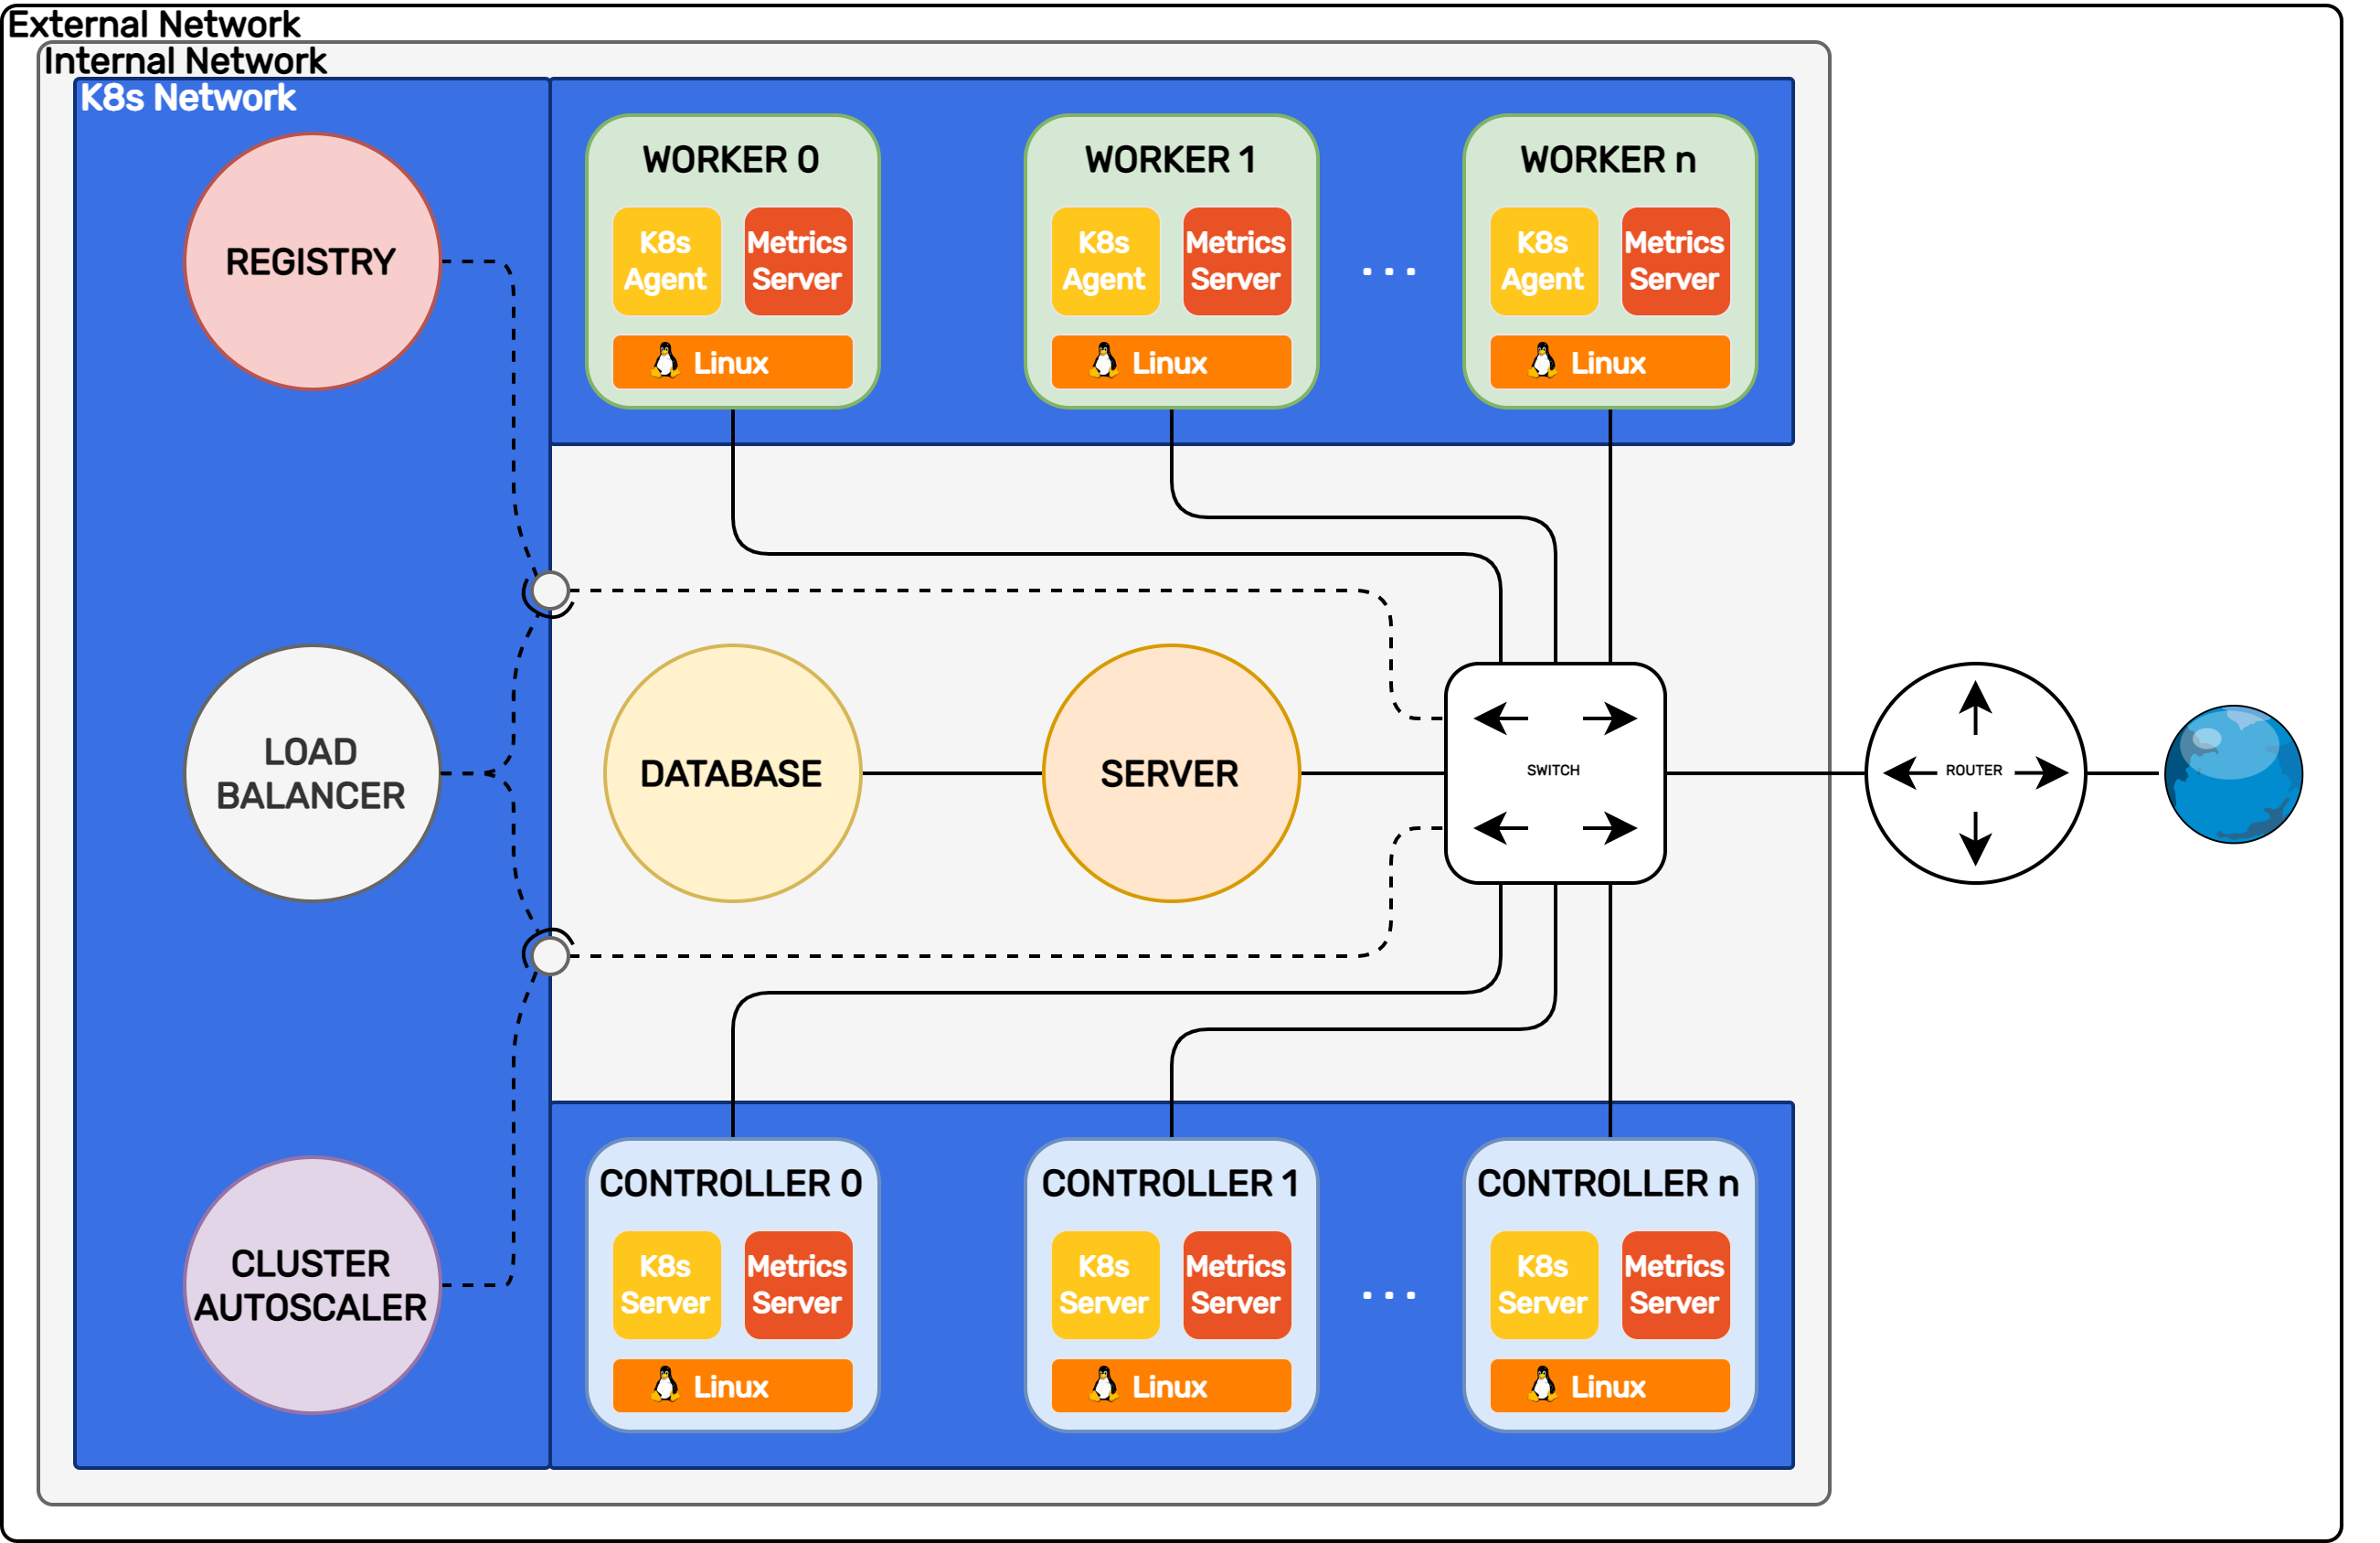
\includegraphics[width=.9\textwidth]{images/recluster/architecture.png}
  \caption{Architecture overview}
\end{figure}

\section{Components}
\label{sec:architecture_components}

\subsection{Node}
\label{subsec:architecture_components_node}

A node is a physical computer that runs the \texttt{Linux Kernel} and constantly
executes software that is specific to the cluster's composition. Linux is a
clone of the operating system Unix\footnote{\url{https://unix.org}}, written from
scratch by Linus Torvalds\footnote{\url{https://wikipedia.org/wiki/Linus_Torvalds}}
with help from a loosely-knit team of hackers across the world. It aims towards
POSIX and Single UNIX Specification compliance\cite{linux}.\\ %
Each node is physically connected to the other nodes via Ethernet and to the
many operating services/components through a virtual network. Section \ref{sec:architecture_network}
goes into further detail about cluster networking. \\ %
A node can be in one of two states. The \texttt{active} state indicates that a node
is turned on and is actively contributing to the cluster. The \texttt{inactive} state,
on the other hand, shows that a node has been turned off and is no longer actively
contributing to the cluster. This does not imply that the node is worthless and
will never be utilized again, but simply that it is no longer required for the current
cluster demand. A node state can be changed manually by switching the power
button on or off, or automatically through the Cluster Autoscaler component,
which monitors the current cluster state. More details about Cluster Autoscaler may
be found in section \ref{subsec:architecture_components_cluster_autoscaler}. \\ %
% TODO Maybe K8s reference section ?
Two core services are continuously operating on each node. The first service is
a Kubernetes-compliant distribution. Kubernetes, also known as K8s, is an open-source
solution for automating containerized application deployment, scaling, and administration\cite{k8s}.
The second service, Metrics Server, is a server that constantly monitors the node,
exposing hardware and operating system metrics. \\ %
Finally, each node is conceptually divided into two types depending on its role in
the cluster: Worker nodes and Controller nodes. These are discussed in the sections
that follow.

\subsubsection{Worker}
\label{subsubsec:architecture_components_node_worker}

\begin{wrapfigure}
  {l}{0pt} %
  \raisebox{0pt}[\dimexpr\height-\baselineskip\relax]{\centering
  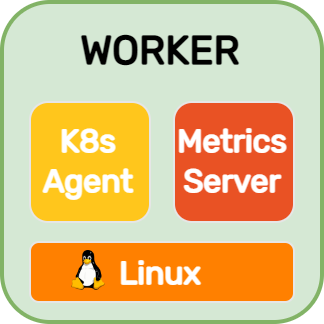
\includegraphics[width=.2\textwidth]{images/recluster/worker.png}}
\end{wrapfigure}

A worker node is designed to handle only deployable units of computation and services
that are not critical components of the cluster. It is not in charge of
scheduling the work over several nodes; rather, it only accepts it from a
cluster-available authenticated and authorized controller node. \\ %
Even though a worker node executes the effectively scheduled workload in the
cluster, it is not considered a critical component of it. At any given time, the
total number of active workers might be zero. That is, there is no scheduled workload,
and previously worker nodes have been shut down automatically to prevent
precious resource waste that is no longer required. \\ %
The majority of the cluster's accessible machines are worker nodes. This raises the
overall amount of schedulable workload as well as heterogeneity. Heterogeneity
is helpful because it may help schedule workloads to nodes with the bare minimum
of requested resources, preventing waste. Assume that the total number of
\texttt{active} nodes in the cluster is zero and that there are two \texttt{inactive}
worker nodes. The first node has 4 GiB of memory and consumes 100W of power,
whereas the second node has 8 GiB of memory and consumes 150W of power. A workload
using around 3GiB of memory is then planned for the cluster. Because it
decreases resource waste, notably memory waste, the first worker node will be
chosen. It is important to note that if both nodes have an equal amount of memory,
the conclusion remains the same since it has the lowest power consumption.

\subsubsection{Controller}
\label{subsubsec:architecture_components_node_controller}

\begin{wrapfigure}
  {l}{0pt} %
  \raisebox{0pt}[\dimexpr\height-\baselineskip\relax]{\centering
  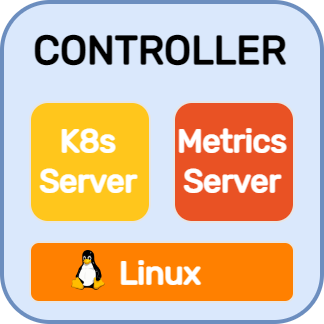
\includegraphics[width=.2\textwidth]{images/recluster/controller.png}}
\end{wrapfigure}

A controller node is an essential component of the cluster, acting as a coordinator
between the active worker nodes and the overall workload in the cluster. It
continually monitors the cluster's state in terms of available nodes, how and where
the workload should be scheduled, and much more. A consistent and secure API must
be provided for administration and end-users who wish to deploy custom services in
the cluster. The API can be made available to an external network if it is
available and appropriately configured, allowing remote control and improving overall
usage. \\ %
To ensure the integrity and management of a cluster, at least one controller
node must be constantly available. It is strongly suggested to have multiple controller
nodes that meet the high availability model to withstand potential system,
component, or application failures. This is possible considering an odd number
of controller nodes (i.e. three) that are always active. A quorum of controller
nodes is required for a cluster to agree on cluster state updates. Quorum in a cluster
with \texttt{n} controllers is \texttt{(n / 2) + 1}. Adding one node to any odd-sized
controller group will always increase the number of nodes required for a quorum.
Although adding a node to an odd-sized controller group appears to improve fault
tolerance since there are more machines, it worsens it because the same number
of nodes can crash without losing quorum but there are more nodes that can fail.
If the cluster cannot withstand any more failures, adding a node before removing
nodes is dangerous because if the new controller node fails to register, the cluster
quorum would be permanently lost\cite{quorum}. The latter is not a strict necessity,
but rather a preferable practice, even though it may slightly increase total resource
waste. Consider this: if the only available controller node encounters a software
or hardware failure and becomes unavailable, the entire cluster becomes
unreachable and unusable.\\ %
To further decrease overall resource waste, a controller can also become a
worker at the same time. If the overall workload in the cluster is very low and non-zero,
having one worker and one controller active with minimal utilization at the same
time is a waste. A single machine can perform the same task, saving precious
resources. If the entire demand grows later and the sole active node becomes overloaded,
the cluster reverts to its previous state. This is a configuration that may be enabled
or disabled based on the management needs of the cluster. \\ %
It should be noted that the total number of active or inactive nodes in the cluster
is not limited. However, a large number of nodes increases the workload on controller
nodes, which must maintain the cluster state updated and synchronized. As a result,
as shown in table \ref{tbl:controller_node_requirements}\cite{k3s_requirements},
their number and hardware requirements must be carefully balanced.

\begin{xltabular}
  {\textwidth} { c | >{\ttfamily}c | >{\ttfamily}c | >{\ttfamily}c }

  \multicolumn{1}{ c |}{\large{\textbf{Deployment Size}}} &
  \multicolumn{1}{ c |}{\large{\textbf{Nodes}}} &
  \multicolumn{1}{ c |}{\large{\textbf{CPU Cores}}} &
  \multicolumn{1}{ c}{\large{\textbf{RAM Memory}}} \\ \hline \hline

  Small & \raisebox{0.5ex}{\texttildelow}10 & 2 & 4 GiB \\ \hline

  Medium & \raisebox{0.5ex}{\texttildelow}100 & 4 & 8 GiB \\ \hline

  Large & \raisebox{0.5ex}{\texttildelow}250 & 8 & 16 GiB \\ \hline

  X-Large & \raisebox{0.5ex}{\texttildelow}500 & 16 & 32 GiB \\ \hline

  XX-Large & 500+ & 32 & 64 GiB \\

  \caption{Controller node requirements based on cluster size}
  \label{tbl:controller_node_requirements}
\end{xltabular}

\subsection{Server}
\label{subsec:architecture_components_server}

\begin{wrapfigure}
  {l}{0pt} %
  \raisebox{0pt}[\dimexpr\height-\baselineskip\relax]{\centering
  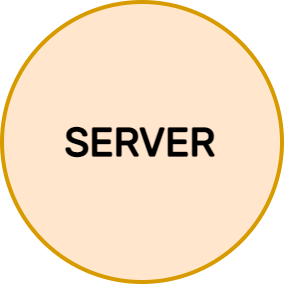
\includegraphics[width=.2\textwidth]{images/recluster/server.png}}
\end{wrapfigure}

A server handles all cluster nodes, user authentication and authorization, and much
more. It does not directly monitor the workload in the same way as a controller
node does, but it does serve as a low-level middleware controller. Every action
is made because of human intervention (e.g., administrators) or another
component of the cluster that has much higher-level knowledge of the current
state and reacts appropriately. \\ %
It is both an essential and a non-essential component of the cluster. It is essential
in the sense that it is aware of all registered nodes, both active and inactive,
and understands how to switch them on and off automatically. It reduces resource
waste by automatically increasing or decreasing the number of nodes in the
cluster when used in conjunction with the Cluster Autoscaler component (see section
\ref{subsec:architecture_components_cluster_autoscaler}). Without prior information,
there is no component in the cluster that can operate as an oracle about the
nodes, leaving the Cluster Autoscaler worthless and increasing total resource waste.
It is also deemed non-essential in the sense that, while decreasing resource waste
is the overall architecture's goal, there is no requirement for a high
availability model as in controller nodes. If a server instance crashes and does
not restart, leaving no more servers in the cluster, the entire cluster continues
to function normally. However, unless failures, human interaction, or server restarts,
the number of active nodes remains constant, potentially increasing resource waste.
\\ %
A server instance does not have to run on a dedicated node. A node can hold
numerous components at the same time, as previously mentioned. A node may be a
server, a controller, and a worker all at the same time, drastically decreasing resource
waste. It is crucial to note, however, that a server should not be executed on a
worker node since, as previously explained, the total number of active workers
might be zero, terminating the server instance and the capability of automatically
adjusting the cluster size. \\ %
The server provides an API to facilitate cluster administration. Furthermore, as
previously said, it is in charge of user authentication and authorization. Unharmful
queries (providing information about active nodes or listing non-sensible
information about a user) should not require any authentication or only a minimal
one. Queries that mutate the state of the cluster or display sensitive
information (turning on or off a node or displaying sensitive user information)
must be protected by a high-security mechanism. \\ %
A heartbeat daemon must be implemented on the server to continuously check the
condition of a node and detect any problems. A heartbeat is a periodic signal or
message created by hardware or software that is sent between devices at regular intervals
of seconds. If the endpoint does not receive a heartbeat for an extended period,
often many heartbeat intervals, the machine that should have sent the heartbeat
is assumed to have failed\cite{heartbeat}. The latter is commonly implemented by
controller nodes since they must constantly monitor and acquire information
about active nodes for workload scheduling. As a result, a server can use the
controller's API to eliminate duplication, increase consistency and availability,
and simplify implementation. \\ %
For more information, section \ref{sec:implementation_server} covers in detail how
the server component is implemented.

\subsection{Database}
\label{subsec:architecture_components_server_database}

\begin{wrapfigure}
  {l}{0pt} %
  \raisebox{0pt}[\dimexpr\height-\baselineskip\relax]{\centering
  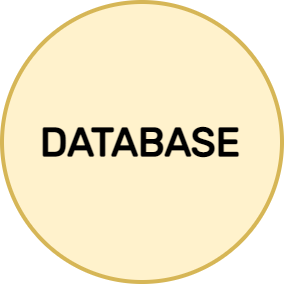
\includegraphics[width=.2\textwidth]{images/recluster/database.png}}
\end{wrapfigure}

The database component is strictly related to the server component. Its primary
function is to store all cluster-related data in a safe, persistent and fault-tolerant
system. The data in question is generally static and does not change frequently.
Static data includes all node-related information, such as CPU type and RAM
quantity, that is hardly modified after the node is added to the cluster.
However, some data, like information regarding the current node state and its
last heartbeat, are intrinsically dynamic in the sense that the system regularly
changes them to ensure integrity. Like the server component, is seen as both necessary
and non-essential. A server is worthless without the database, resulting in the same
outcome as previously explained. \\ %
This component is seen as the union of numerous modules that form it rather than
as a single entity. A database, in general, is a structured collection of
information or data that is persistently stored in a computer system. A database
management system (DBMS) is a software program that acts as an interface between
the database and its end users or applications, allowing for the retrieval, updating,
and administration of how information is structured and optimized. A DBMS also facilitates
database supervision and control by providing several administrative operations such
as performance monitoring, tuning, and backup and recovery\cite{database}. The latter
indicates that each module and feature is dependent on the implementation. Only
for the database itself, there are several distinct types, and for each type, there
are numerous distributions with varying features and capabilities. To better
follow the overall design criteria, the ultimate decision on which one to take must
be carefully examined. \\ %
Persistency and fault tolerance are strongly related, most importantly, in the data
layer. Even if an error occurs, the only vital and critical component that must be
preserved and not lost is all the stored data. Data persistency is the
preservation of data after the program that produced it has been terminated. To do
this, the data must be written to non-volatile storage, a type of memory that can
maintain the information indefinitely even if the program is no longer functioning\cite{persistency}.
Fault tolerance, which differs slightly from the previous definition, refers to a
non-volatile storage system's capacity to recover from an error or faulty condition,
most typically an irreversible hardware failure of some type, without losing any
previously stored data. Disk fault tolerance is often achieved by disk
management technologies such as mirroring\footnote{\url{https://wikipedia.org/wiki/Disk_mirroring}},
data striping\footnote{\url{https://wikipedia.org/wiki/Data_striping}},
duplexing\footnote{\url{https://www.pcmag.com/encyclopedia/term/disk-duplexing}},
and Redundant Array of Independent (or Inexpensive) Disks (RAID)\footnote{\url{https://wikipedia.org/wiki/RAID}}\cite{disk_management_technologies}.
Consider the possibility that the database component has a hardware failure and ceases
to operate. The damage has compromised not just the replaceable hardware (such as
the CPU, motherboard, and RAM), but also some (but not all) storage devices storing
the cluster's data. Typically, all data is irreversibly lost, and the cluster
must be rebuilt from scratch. However, with a correctly designed disk management
system, once the faulty hardware is replaced, all data is automatically
recovered and the cluster becomes functional again. The process of rebuilding the
data might take a significant amount of time (i.e. calculating the parity bit\footnote{\url{https://wikipedia.org/wiki/Parity_bit}}).
\\ %
Finally, an optional cache middleware can be implemented between the server and database,
enhancing read speed for frequently requested but rarely updated data and
reducing disk utilization. The cached data is stored in the main volatile memory.

\subsection{Registry}
\label{subsec:architecture_components_registry}

\begin{wrapfigure}
  {l}{0pt} %
  \raisebox{0pt}[\dimexpr\height-\baselineskip\relax]{\centering
  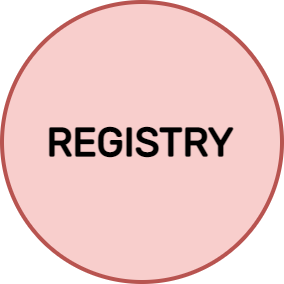
\includegraphics[width=.2\textwidth]{images/recluster/registry.png}}
\end{wrapfigure}

\subsection{Cluster Autoscaler}
\label{subsec:architecture_components_cluster_autoscaler}

\begin{wrapfigure}
  {l}{0pt} %
  \raisebox{0pt}[\dimexpr\height-\baselineskip\relax]{\centering
  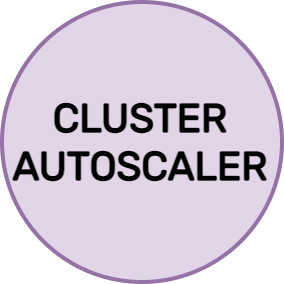
\includegraphics[width=.2\textwidth]{images/recluster/cluster_autoscaler.png}}
\end{wrapfigure}

\subsection{Load Balancer}
\label{subsec:architecture_components_load_balancer}

\begin{wrapfigure}
  {l}{0pt} %
  \raisebox{0pt}[\dimexpr\height-\baselineskip\relax]{\centering
  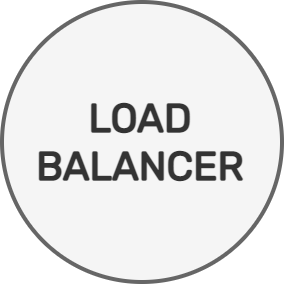
\includegraphics[width=.2\textwidth]{images/recluster/load_balancer.png}}
\end{wrapfigure}

\section{Network}
\label{sec:architecture_network}

\subsection{Overlay Network}
\label{subsec:architecture_network_overlay_network}

\subsection{Domain}
\label{subsec:architecture_network_domain}

\section{Cluster}
\label{sec:architecture_cluster}

\begin{wrapfigure}
  {r}{.5\textwidth}
  \centering
  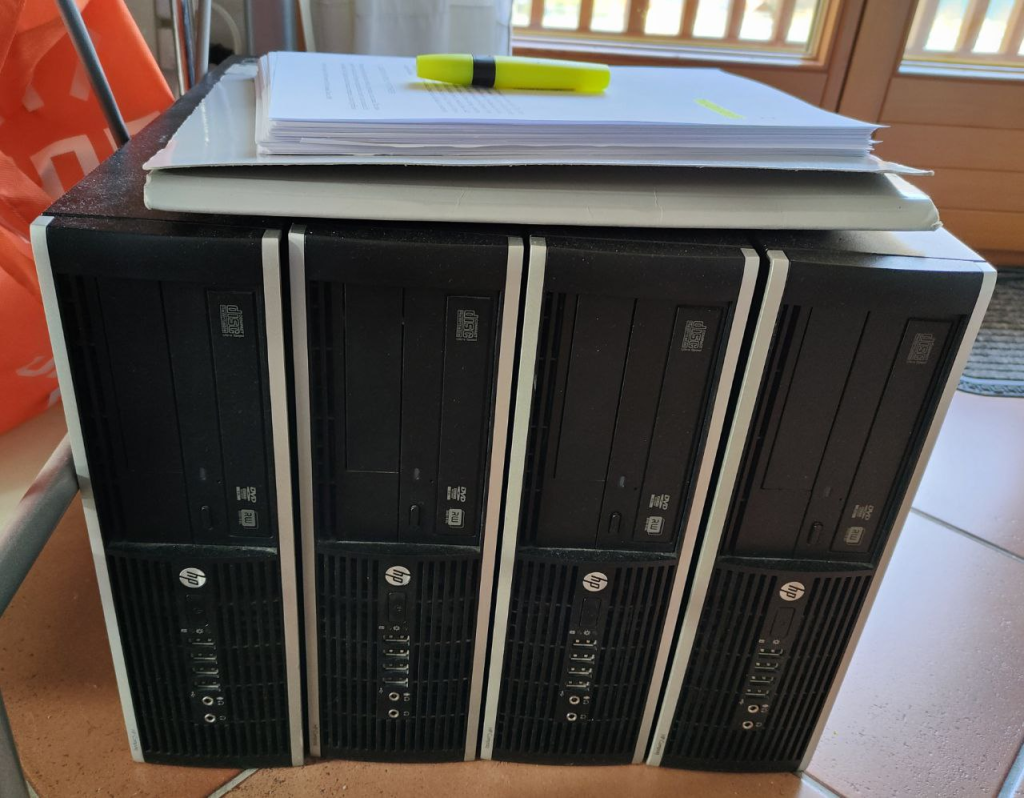
\includegraphics[width=.5\textwidth]{images/recluster/cluster.png}
  \caption{reCluster cluster}
\end{wrapfigure}

\subsection{Hardware}
\label{subsec:architecture_cluster_hardware}

% TODO WoL features, how to turn on nodes
% TODO Prefer nodes with WoL upscaling

\subsection{Example}
\label{subsec:architecture_cluster_example}

% TODO Move
  \chapter{Implementation}
\label{cha:implementation}

\epigraph{Ideas are easy, Implementation is hard.}{Guy Kawasaki}

Most of the implementation details and general decisions made for developing a
real-world functional project, based on the design architecture presented in chapter
\ref{cha:architecture}, are discussed in this chapter. It is organized in such a
way that it starts with the foundation and then progresses to the autoscaling of
worker nodes before moving on to example deployments of various applications in the
cluster. \\ %
The technology and programming languages utilized in the implementation are heterogeneous.
Nevertheless, according to a shared set of APIs and pre-defined structures, they
interact as a distinct and homogenous entity that maintains the entire cluster
in an active and healthy state. \\ %
Furthermore, several of the components and/or technologies discussed in this chapter
are interchangeable with other solutions. The latter is highly valuable for
organizations since it provides more configuration freedom and final control
over the cluster while continuously reflecting its ultimate goal.

\section{Distributions}
\label{sec:implementation_distributions}

% TODO Reference introduction dependencies

Almost all software relies on the necessity for a stable and consistent
operating system (OS). \\ %
The OS, as specified in section \ref{subsec:architecture_components_node}, is
installed on every node in the cluster and must be based on the \texttt{Linux
Kernel}. The latter is a critical requirement because most of the technologies
employed in the implementation rely on Linux primitives and core functionality
to operate properly. To enforce resource management for pods and containers, for
example, all Kubernetes distributions require the \texttt{cgroup v2}\footnote{\url{https://www.kernel.org/doc/html/latest/admin-guide/cgroup-v2.html}}
kernel module\footnote{\url{https://kubernetes.io/docs/concepts/architecture/cgroups}}.
Furthermore, the Linux Kernel is an Open Source project to which everyone can
contribute and get access, representing one fundamental objective of the entire project.
\\ %
To represent the potential of the implementation architecture being compatible with
several Linux distributions, the section is titled Distributions rather than
Operating System. A Linux distribution, often known as a Linux distro, is an operating
system that is built from components developed by various open-source projects and
programmers. The Linux kernel (the operating system's core), the GNU shell utilities
(terminal interface and commands), the X server (for a graphical desktop), the desktop
environment, a package management system, an installer, and other services are
all included in each distribution. Many components are created independently and
released in source code format. Thousands of software packages, utilities, and
applications can be found in a single Linux distribution. Linux distributions combine
code from open-source projects into a single operating system that can be installed
and booted. Linux distributions are available for a wide range of specialized
use cases, including desktop computers, servers without a graphical interface, supercomputers,
mobile devices, and more\cite{linux_distro}. \\ %
To be completely compatible with the implementation architecture, a Linux distribution
must meet three major requirements. They are described in the following list:
\begin{enumerate}
  \item The Linux Kernel version must be compatible with the Kubernetes version.
    \newline
    Newer versions of K8s may require newer versions of the Linux Kernel to
    provide newer functions and/or improve overall security.

  \item All necessary packages, as explained and documented in the section
    \ref{subsec:implementation_distributions_packages}, must be installed and globally
    accessible in the system.
    \newline
    A check on all essential packages is performed before the execution of the
    installation program, as detailed in section \ref{sec:implementation_installer}.
    If even one package is missing from the system, the installation fails with an
    error message identifying the missing packages.

  \item An Init System that is supported and compatible, as defined in the
    section \ref{subsec:implementation_distributions_init_system}.
    \newline
    OpenRC and Systemd are supported by the implementation. They are currently
    the two most used init systems, and the majority of available distributions are
    based on one of them.
\end{enumerate}
Finally, two custom Linux distributions are already configured, built, and
packaged as ISO files, as shown in section \ref{subsec:implementation_distributions_iso_image}.
They are based on a simple command line with no graphical interface and contain
only what is required to start a node. This is done to simplify the overall setup
by eliminating unnecessary software and technologies, addressing any
incompatibilities, and increasing the cluster's implementation and testing efficiency.
Both are derived from pre-existing Linux distributions that are known to be
stable, easy to configure, and lightweight, requiring just the bare minimum of resources
to operate. Furthermore, they are built on separate init systems, requiring the
overall implementation to be compatible with and tested with both.

\subsection{Packages}
\label{subsec:implementation_distributions_packages}

\subsection{Init System}
\label{subsec:implementation_distributions_init_system}

\subsubsection{OpenRC}
\label{subsec:implementation_distributions_init_system_openrc}

\subsubsection{Systemd}
\label{subsec:implementation_distributions_init_system_systemd}

\begin{wrapfigure}
  {r}{.25\textwidth}
  \centering
  
\includegraphics[width=.25\textwidth]{images/logos/systemd.png}
  \caption{Systemd logo}
\end{wrapfigure}

\subsection{ISO image}
\label{subsec:implementation_distributions_iso_image}

\subsubsection{Generation}
\label{subsubsec:implementation_distributions_iso_generation}

\subsubsection{Alpine Linux}
\label{subsubsec:implementation_distributions_iso_alpine_linux}

\begin{wrapfigure}
  {r}{.25\textwidth}
  \centering
  
\includegraphics[width=.25\textwidth]{images/logos/alpine.png}
  \caption{Alpine Linux logo}
\end{wrapfigure}

Alpine Linux\footnote{\url{https://www.alpinelinux.org}} is a lightweight,
security-focused, and resource-efficient distribution. In recent years, has grown
in popularity as the foundation for the majority of Docker images. It is based
on musl\footnote{\url{https://musl.libc.org}} (an implementation of the C standard
library, an alternative to glibc), BusyBox\footnote{\url{https://busybox.net}} (a
single, small executable that combines tiny versions of many common UNIX
utilities), a custom package manager called APK\footnote{\url{https://wiki.alpinelinux.org/wiki/Alpine_Package_Keeper}}
and the OpenRC init system ()\cite{alpine_linux}. \\ % TODO OpenRC reference
Alpine Linux is the preferred reCluster distribution. It has been utilized and tested
during development and is now present in every cluster node.

\subsubsection{Arch Linux}
\label{subsubsec:implementation_distributions_iso_arch_linux}

\begin{wrapfigure}
  {r}{.25\textwidth}
  \centering
  
\includegraphics[width=.25\textwidth]{images/logos/arch.png}
  \caption{Arch Linux logo}
\end{wrapfigure}

Arch Linux\footnote{\url{https://archlinux.org}} is a general-purpose distribution
that focuses on simplicity, minimalism, and code elegance. It is based on
Systemd init system () % TODO Systemd reference
and strives to stay bleeding edge, offering the latest stable versions of most software
through Pacman\footnote{\url{https://wiki.archlinux.org/title/Pacman}} package manager.
Uses a rolling release system that allows one-time installation and perpetual
software upgrades, allowing to not reinstall or upgrade the system from one version
to the next. Notably, Arch Linux is the foundation for several many popular enterprise-grade
distributions, such as Manjaro\footnote{\url{https://manjaro.org}} and SteamOS\footnote{\url{https://store.steampowered.com/steamos}},
demonstrating its customizability, power, and stability\cite{arch_linux}.

\section{Dependencies}
\label{sec:implementation_dependencies}

% TODO Dependencies presentation

\subsection{Air-Gap Environment}
\label{subsec:implementation_dependencies_air_gap_environment}

\subsection{Management}
\label{subsec:implementation_dependencies_management}

\subsubsection{Configuration}
\label{subsec:implementation_dependencies_management_configuration}

\subsubsection{Script}
\label{subsec:implementation_dependencies_management_script}

\subsection{K3s}
\label{subsec:implementation_dependencies_k3s}

\begin{wrapfigure}
  {r}{.25\textwidth}
  \centering
  
\includegraphics[width=.25\textwidth]{images/logos/k3s.png}
  \caption{K3s logo}
\end{wrapfigure}

\subsection{Node Exporter}
\label{subsec:implementation_dependencies_node_exporter}

\subsection{Prometheus}
\label{subsec:implementation_dependencies_prometheus}

\begin{wrapfigure}
  {r}{.25\textwidth}
  \centering
  
\includegraphics[width=.25\textwidth]{images/logos/prometheus.png}
  \caption{Prometheus logo}
\end{wrapfigure}

\subsection{Autoscaler}
\label{subsec:implementation_dependencies_autoscaler}

\subsubsection{Cluster Autoscaler}
\label{subsec:implementation_dependencies_autoscaler_cluster_autoscaler}

\section{Installer}
\label{sec:implementation_installer}

\subsection{POSIX Shell}
\label{subsec:implementation_installer_posix_shell}

\subsection{Configuration Arguments}
\label{subsec:implementation_installer_configuration_arguments}

\subsection{Configuration Files}
\label{subsec:implementation_installer_configuration_files}

\subsubsection{Certificates}
\label{subsubsec:implementation_installer_configuration_files_certificates}

\subsubsection{K3s}
\label{subsubsec:implementation_installer_configuration_files_k3s}

\subsubsection{K8s}
\label{subsubsec:implementation_installer_configuration_filesn_k8s}

\subsubsection{Node exporter}
\label{subsubsec:implementation_installer_configuration_files_node_exporter}

\subsubsection{reCluster}
\label{subsubsec:implementation_installer_configuration_files_recluster}

\subsubsection{SSH}
\label{subsubsec:implementation_installer_configuration_files_ssh}

\subsection{Node Facts}
\label{subsec:implementation_installer_node_facts}

\subsection{Node Information}
\label{subsec:implementation_installer_node_information}

\subsection{Node Benchmarks}
\label{subsec:implementation_installer_node_benchmarks}

\subsubsection{SysBench}
\label{subsubsec:implementation_installer_node_benchmarks_sysbench}

\subsection{Node Power Consumption}
\label{subsec:implementation_installer_node_power_consumption}

\subsubsection{CloudFree Smart Plug}
\label{subsubsec:implementation_installer_node_power_consumption_cloudfree_smart_plug}

\subsection{Node Registration}
\label{subsec:implementation_installer_node_registration}

\subsubsection{K8s Node Label And Name}
\label{subsubsec:implementation_installer_node_registration_k8s_node_label_and_name}

\subsection{Cluster Initialization}
\label{subsec:implementation_installer_cluster_initialization}

\subsubsection{Kubeconfig}
\label{subsubsec:implementation_installer_cluster_initialization_kubeconfig}

\subsubsection{Database}
\label{subsubsec:implementation_installer_cluster_initialization_database}

\subsubsection{Server}
\label{subsubsec:implementation_installer_cluster_initialization_server}

\subsubsection{Admin And Autoscaler Users}
\label{subsubsec:implementation_installer_cluster_initialization_admin_and_autoscaler_users}

\subsubsection{K8s}
\label{subsubsec:implementation_installer_cluster_initialization_k8s}

\subsection{Services}
\label{subsec:implementation_installer_services}

\subsubsection{Start}
\label{subsubsec:implementation_installer_services_start}

\subsubsection{Stop}
\label{subsubsec:implementation_installer_services_stop}

\subsubsection{Boot}
\label{subsubsec:implementation_installer_services_boot}

\subsubsection{Shutdown}
\label{subsubsec:implementation_installer_services_shutdown}

\section{Server}
\label{sec:implementation_server}

\subsection{Database}
\label{subsec:implementation_server_database}

\subsubsection{PostgreSQL}
\label{subsubsec:implementation_server_database_postgresql}

\begin{wrapfigure}
  {r}{.25\textwidth}
  \centering
  
\includegraphics[width=.25\textwidth]{images/logos/postgresql.png}
  \caption{PostgreSQL logo}
\end{wrapfigure}

\subsubsection{Prisma}
\label{subsubsec:implementation_server_database_prisma}

\begin{wrapfigure}
  {r}{.25\textwidth}
  \centering
  
\includegraphics[width=.25\textwidth]{images/logos/prisma.png}
  \caption{Prisma logo}
\end{wrapfigure}

\subsubsection{Schema}
\label{subsubsec:implementation_server_database_schema}

\subsection{GraphQL}
\label{subsec:implementation_server_graphql}

\subsubsection{GraphQL vs REST}
\label{subsubsec:implementation_server_graphql_graphql_vs_rest}

\subsubsection{Schema}
\label{subsubsec:implementation_server_graphql_schema}

\subsection{Node Pool}
\label{subsec:implementation_server_node_pool}

\subsection{Node Registration}
\label{subsec:implementation_server_node_registration}

\subsubsection{JSON Web Token}
\label{subsubsec:implementation_server_node_registration_json_web_token}

\subsection{Upscaling}
\label{subsec:implementation_server_upscaling}

\subsubsection{Wake-on-LAN}
\label{subsubsec:implementation_server_scale_up_wake_on_lan}

\subsection{Downscaling}
\label{subsec:implementation_server_downscaling}

\subsubsection{SSH}
\label{subsubsec:implementation_server_scale_up_ssh}

\section{Autoscaling}
\label{sec:implementation_autoscaling}

\subsection{Vertical Pod Autoscaler}
\label{subsec:implementation_autoscaling_vertical_pod_autoscaler}

\subsection{Horizontal Pod Autoscaler}
\label{subsec:implementation_autoscaling_horizontal_pod_autoscaler}

\subsection{Cluster Autoscaler}
\label{subsec:implementation_autoscaling_cluster_autoscaler}

\subsubsection{Cloud Provider}
\label{subsubsec:implementation_autoscaling_cluster_autoscaler_cloud_provider}

\subsubsection{Configuration}
\label{subsubsec:implementation_autoscaling_cluster_autoscaler_configuration}

% TODO Cloud Configuration

\subsubsection{Upscaling}
\label{subsubsec:implementation_autoscaling_cluster_autoscaler_upscaling}

\subsubsection{Downscaling}
\label{subsubsec:implementation_autoscaling_cluster_autoscaler_downscaling}
  \chapter{Analysis}
\label{cha:analysis}

\section{Difficulties}
\label{sec:analysis_difficulties}

\section{Criticalities}
\label{sec:analysis_criticalities}

\section{Limitations}
\label{sec:analysis_limitations}

\section{Shortcomings}
\label{sec:analysis_shortcomings}

\subsection{Graphical User Interface}
\label{subsec:analysis_shortcomings_graphical_user_interface}


  % Conclusions
  \chapter{Conclusions}
\label{cha:conclusions}

Current cluster architectures are mainly concerned with maximizing service performance
and achieving near-instantaneous responsiveness while ignoring the energy impact
and the various resources involved. As a result, it is becoming more and more necessary---almost
a requirement---to reconsider and transform existing designs to create architectures
that are more resource-aware and sustainable. These latter requirements must be
considered just as vital as performance and responsiveness. \\ %
The context and fundamental principles on which the new and more sustainable
cluster architectures should either completely or partially rely on have been
initially explained in this document. Moreover, due to the outsourcing
phenomenon that shifts local and physical architectures towards remote, intangible,
and virtual architectures, users tend to forget the numerous implications of this
decision that not only can have privacy and/or security concerns but also, and
most importantly in this case, completely removes the direct control and the resource
awareness of the overall system. \\ %
Following the introduction, a possible theoretical design that is more
sustainable has been put forward, prioritizing the reduction of resource waste and
energy consumption while maintaining a certain degree of adaptability and configurability.
Every component that constitutes the architecture has been thoroughly explained,
highlighting its main purpose and different capabilities. A cluster is not a
cluster if the different components are not connected. In the design, there are
three major network groups; the External Network may even be removed if external
resources and connections are not required. The reCluster project, which is a practical
and sustainable cluster implementation of the theorized architecture, has also
been presented. All of its hardware components have been recycled following decommissioning.
\\ %
The implementation thoroughly explains how the reCluster was put into practice while
adhering to both the fundamental requirements and the theoretical architecture behind
the networks and components. It begins with the foundations, which are composed of
GNU/Linux, a collection of programs, and the Init System, all of which are
packaged together as a custom distribution into a portable and simple-to-install
ISO image file. Then, each theorized component is mapped to a real-world
application, and some of its most important features used in reCluster are explained.
The way the Server and Cluster Autoscaler components are implemented is
different because the first one was entirely built from scratch, whereas the second
one used an existing core that had been modified to be compatible with the cluster
version. The Server component represents the low-level knowledge of the cluster
and is deeply described, including the database structure, GraphQL queries and
mutations API, how the upscaling and downscaling procedures are handled, and how
to exploit Kubernetes monitoring without the need for a custom implementation. The
Cluster Autoscaler, on the other hand, represents the high-level knowledge of the
cluster, and it is used in conjunction with the Server component to perform the
upscaling or downscaling operations. The Cluster Autoscaler only scales the number
of nodes and, because it is not the only method of autoscaling in a cluster, the
other two approaches are also explained: Vertical Pod Autoscaler, which automatically
adjusts the resources of a Pod, and Horizontal Pod Autoscaler, which automatically
adjusts the number of Pods. The combination of the Horizontal Pod Autoscaler and
the Cluster Autoscaler is critical for improving total automation and minimizing
the need for human intervention, as well as lowering overall power consumption while
maintaining scalability. \\ %
Lastly, because manually installing the cluster and providing all of the
necessary information is tedious, the installation script that automatically performs
the installation operation while following a specific set of configuration parameters
has been discussed and proposed. Moreover, it is demonstrated how the node's benchmarks
and power consumption data are measured. Finally, the most essential elements of
the configuration and deployment files of the various components and/or technologies
used are illustrated and discussed, so that the employed features of each can be
recognized. \\ %
With all of the prior information and technology, building and deploying a more sustainable
and resource-aware cluster is feasible without incurring into breaking trade-offs;
while it may be regarded as a tiny step towards greener computing, it, along
with other initiatives, attempts to bring the end result closer to realization.

\section{Limitations And Future Work}
\label{sec:conclusions_limitations_and_future_works}

This section depicts some of the difficulties encountered, existing criticalities
and limitations, and relevant future ideas that can enhance and extend the
current architecture and implementation. Because one of the project's main points
is FOSS (Free and Open Source Software) compliance, anyone from anywhere can
contribute to it. The latter not only can increase the overall number of features
but also improve overall stability thanks to intrinsic testing in various use-case
scenarios and heterogeneous environments, which allows for the discovery and
correction of previously unknown bugs and/or errors. External contributions from
a wide variety of users are so valuable that they are frequently undervalued and
underestimated in current contexts. \\ %

The combination of the installation script and the external device for measuring
power consumption only conducts simple and basic readings on the instantaneously
drawn energy. This is ideal for desktop computers and servers that require an external
energy source, but it is incompatible with devices that use an internal energy
source (batteries), such as laptop computers. \\ %
If the existing implementation of the installation script is executed on a laptop
computer, the resulting power consumption readings are inaccurate since it does
not take into consideration the current absorbed energy from both the external (plug)
and internal (battery) sources, but only the first. As a result, the obtained final
power consumption data are always lower than what are in reality, leading to
general inefficiency and erroneous selection by the algorithm in upscaling and
downscaling operations, because the Server recognizes the node as a much more power-efficient
system than it is. \\ %
The script should determine whether the current node has internal energy sources
and, when conducting power consumption readings and calculations, adjust with a more
sophisticated but efficient and compatible algorithm that takes into account for
both external and internal absorbed energy. Moreover, further testing on devices
with an internal energy source is required to better understand how the system is
powered, as it can solely use the external source, only use the internal source,
or even employ both. \\ %

Another of the project's most significant difficulties has been developing the recluster
Cloud Provider for the Cluster Autoscaler. There are three primary reasons for
this. \\ %
First off, the Cluster Autoscaler and the majority of the Kubernetes development
environment are built using the Go\footnote{\url{https://go.dev}} programming language.
I had never written a line of Go code before developing the \texttt{recluster} Cloud
Provider, so I had to learn the language from the beginning as well as the
package ecosystem, code style, and syntax. Although difficult at first, the
effort paid off in the end. \\ %
Second, neither official nor unofficial documentation exists that explains how to
create a Cloud Provider for the Cluster Autoscaler. My entire knowledge of
developing the \texttt{recluster} Cloud Provider is based on studying and evaluating
the code developed by the other Cloud Providers. Additionally, because each Cloud
Provider has a unique implementation, distinct Server logic, and a different API,
I had to determine the similarities and fundamental elements that almost all of
them share to transform it and make it compatible with reCluster. The lack of documentation
is understandable given that only a small number of entities utilize and develop
this technology, making it possible for them to access experts and/or
specialized consulting from the main CA developers themselves. Keep in mind that
the latter needs familiarity with the Go programming language, which was covered
in the preceding point. \\ %
Finally, it took longer than I anticipated to test the Cluster Autoscaler in conjunction
with the Server and the general architecture since almost every time a new,
minor error or bug that I hadn't considered appeared. However, the latter was
not only beneficial for reCluster; it additionally helped in identifying an issue\footnote{\url{https://github.com/kubernetes/autoscaler/issues/5378}}
in the Cluster Autoscaler's main code, which was submitted to the maintainers
and promptly fixed within a week. \\ %

Currently, the only way for a user or administrator to interact with the cluster
is to use applications such as \texttt{curl}, \texttt{wget}, or similarities to
directly use the various set of GraphQL queries and mutation API, or use the GraphQL
Studio Explorer, which is not available in production and is only a nicer
interface for low-level interactions with the GraphQL API. As a result, there is
a need to create a UI dashboard, such as the one from Kubernetes\footnote{\url{https://kubernetes.io/docs/tasks/access-application-cluster/web-ui-dashboard}},
where all of the information provided by the Server is visually available
without involving the user in low-level GraphQL API interactions. The majority of
operations should be simple and intuitive, without needing the user to better
understand the requirements and outcomes. \\ %
Because the web application must consider the authentication mechanism, only authorized
and/or authenticated users may access specific information or do certain operations.
Furthermore, to provide a better overview of all the information accessible to the
user, the dashboard should be capable of generating faster-to-understand graphs
and/or charts. Consider a pie chart in which the number of active/working nodes (green
color) is visually compared against the number of inactive nodes (gray color).
The user can immediately understand the current cluster capacity/demand, where if
the chart is almost entirely green, there is an overall high workload in the
cluster, whereas if the chart is almost entirely gray, there is an overall low
workload in the cluster, and thus the number of inactive nodes predominates. \\ %
With so many tools, technologies, and frameworks available for developing a web application
nowadays, the most difficult and critical phase is choosing which one to use
before even beginning development. \\ %
Also, there may be a desire to improve the simplicity with which each node is managed
without directly requiring \texttt{SSH} or similar technologies. \\ %
The latter can be accomplished by directly integrating a protected graphical
dashboard on each node that displays the various information of the associated
node as well as the ability to install, upgrade, or delete packages and perform
additional operations. \\ %
\texttt{YunoHost}\footnote{\url{https://yunohost.org}}, which leverages a simple
and easy-to-use, but incredibly powerful, web UI dashboard to completely
administer the node, is a starting point for what may be accomplished or developed.
\\ %

Computers are the only systems that are currently used and supported in the
cluster. But, there are an enormous number of unused smartphone and tablet
devices that might be employed in the cluster. Most of these devices are ideal for
becoming worker nodes in a cluster because the previous owners replaced them due
to an upgrade to a newer model or because there is hardware damage, such as on
the screen or camera, but this has not affected important components such as the
main board. Furthermore, these devices have become so powerful in recent years that
they may be compared to the same performance as medium/low-end PCs while having a
significantly lower power consumption thanks to different internal architecture and
a prior design on energy consumption optimizations. \\ %
Developing for mobile devices might be challenging since there may be incompatibilities
between the software used for the cluster related to the internal Operating System
and missing libraries or Kernel requirements. A viable alternative is to
uninstall the existing operating system (\texttt{Android} or \texttt{iOS}) and
replace it with a pure GNU/Linux distribution designed exclusively for mobile
devices, such as \texttt{postmarketOS}\footnote{\url{https://postmarketos.org}}.
It should be noted that the overall compatibility of the Operating System with the
device varies from device to device, and the OS may need to be patched. Mobile development
should not be hard, however, this is the current status and/or only method for quickly
porting applications designed for GNU/Linux on PCs to mobile devices. \\ %
As previously stated, the power consumption of mobile devices is extremely small
compared to what they can provide. When compared to desktop computers and even laptop
computers, the performance-to-power-consumption ratio is enormous. There are no simple
techniques for remotely powering on a mobile device that does not involve custom
solutions. However, it should be mentioned that the sleep mode of mobile devices
is so efficient that a device in sleep mode consumes almost zero energy and may last
for more than a week on a single charge. As a result, if the remote wake-up solution
is too expensive or unfeasible, the concept of keeping a mobile device
constantly in sleep mode might be considered. \\ %

The cluster currently supports only \texttt{amd64} and \texttt{arm64} architectures.
Because the majority of the employed software and technologies support a wide
range of different architectures by default, such as \texttt{mips}\footnote{\url{https://wikipedia.org/wiki/MIPS_architecture}}
or \texttt{mipsel}, the remaining incompatible components, such as the Cluster Autoscaler,
can be ported and/or transformed to be compatible with additional and different
architectures. \\ %
Expanding the number of supported architectures allows more devices to be
incorporated into the cluster, giving them new life while also improving the cluster's
overall workload capacity. \\ %

The existing Node selection algorithm is effective, but it is a simplistic implementation
because it just depends on maximum and minimum power consumptions and, if both
are identical, falls back to performance data. \\ %
The existing algorithm works, despite its simplicity and limited accessible data
to perform all conceivable computations and evaluations. Nevertheless, there are
several aspects where it may be refined to accomplish a more suitable node's
final decision. As an example, while upscaling, the chosen node may have a lower
power consumption and possibly greater performance, whereas when downscaling, it
may have higher power consumption and potentially worse performance. Furthermore,
in future versions, the more efficient and sophisticated algorithm should take
into consideration other factors with a more advanced internal logic. There may be
nodes that are more efficient while under medium workload conditions, while
others that are less efficient when under the same conditions but with lower
minimum and maximum power consumption coefficients. The existing approach is deterministic,
always preferring the second node type when upscaling and the first node type
when downscaling. The new algorithm should perform extra computations and evaluations
on which node type should bootstrap or terminate, and it's expected to follow
the current overall cluster state as well as its overall power consumption. \\ %
The algorithm may also be enhanced with a Kalman Filter\footnote{\url{https://wikipedia.org/wiki/Kalman_filter}}
for estimating the combination of power consumption and workload to
significantly reduce total (real) power consumption while also improving overall
Quality of Service (QoS). \\ %
The latter are merely possible ideas for what the new enhanced algorithm should
include and what possible advancements, such as lowering power consumption while
increasing overall performance, must be addressed. \\ %

There are no graphs or charts in this document to demonstrate how the generally existing
cluster implementation performs on different workloads and/or hardware. This is
because the time and resources required to conduct such measurements accurately
and precisely are presently insufficient for a single person. \\ %
The cluster's performance management can be proposed as an extra document/paper
that not only illustrates the various data collected, but also enhances and extends
the existing design and algorithms with improvements determined from the performance
management results. This task is currently assigned to another CRIT team member
who employs this document as a foundation to better comprehend how the general
architecture is designed and how to obtain correct and precise performance
measurements. \\ %
Even though this document lacks data on performance measurements, the current cluster
implementation by default exposes data that can be used for analysis of general performance
and resource utilization. Every node in the cluster provides real-time hardware
and OS-related data thanks to the Node Exporter component, which is described in
section \ref{subsec:implementation_dependencies_node_exporter}. These metrics
are then collected and analyzed by the Prometheus component, as described in section
\ref{subsubsec:implementation_dependencies_prometheus_features}, which allows
for monitoring and querying/interpolating them with various results that can
cover a specified period. \\ %
Furthermore, because the overall architecture is already established and deployed
automatically, control of overall performance may be employed not only
occasionally or during testing but always. This not only gives reacher statistics,
but it additionally has the potential to provide real-time alerts on the overall
health of the cluster. Besides that, custom notifications that monitor the total
cluster power consumption can be established. This can be critical in a variety of
use-case situations. Consider the following scenario: the cluster is powered solely
by batteries that are charged during the day by solar panels, similar to the Low-Tech
magazine\footnote{\url{https://solar.lowtechmagazine.com}}, and there is a known
overall threshold amount of energy consumption that, if exceeded, can cause the entire
cluster to go offline until the next recharge. Employing an accurate performance
management system to compute the threshold, as well as a monitoring and alerting
system to notify an administrator, is critical; enabling the cluster to be online
and active as much as possible while also performing its main routine of service
orchestration. \\ %
Nevertheless, this point is critical, and it must be addressed and implemented in
future versions of reCluster. \\ %

In addition to the preceding point, there is a missing section where the various
use-case scenarios are analyzed and tested owing to the same reasons of a single
person's lack of time and resources. \\ %
Currently, only two use-case scenarios have been successfully evaluated in a
real-world context using the reCluster cluster architecture. The first scenario is
a one-to-one mapping to a potential cluster used for hosting various services that
need to be exposed to an external network or, more broadly, the Internet. It has
a stable connection, and most of the components and their configurations may be downloaded,
guaranteeing the most recent and up-to-date versions are used in the cluster. Having
the most recent versions available might be beneficial since there may be bugs or
security vulnerabilities that have been addressed, whereas the bundled ones may
contain issues due to being outdated. The first scenario is the most common, in
which practically anybody can deploy a cluster without difficulty. The second scenario,
on the other hand, is an Air-Gap environment in which there is no Internet connection
and all components and processes must be available and performed offline. The
latter has been well detailed throughout the document, and it may also be regarded
as a solid foundation/requirement for future environmental and availability crises
in which having an internet connection is no longer obvious. Using Air-Gap
measurements only during the installation procedure, while the normal execution is
in normal conditions with an Internet connection, can be advantageous because it
does not require any download, reducing overall installation time and also avoiding
the involvement of networking equipment, which can consume unnecessary energy, and
the installed software behavior is always predictable. \\ %
In addition to the preceding two scenarios, the cluster might be deployed in two
additional scenarios. The first instance is when the cluster may be used in education
to evaluate students' work. The latter can be employed to test their Kubernetes abilities,
as well as teach them basic and advanced web apps or APIs that include various
software components, such as a server, a database, and a cache server. The
second scenario is for redundancy, in which reCluster is being used only if the main
cluster, which is more performant but consumes more energy, is no longer accessible
due to a failure. reCluster uses decommissioned main cluster hardware and has
just one Controller node active, whereas all worker nodes are inactive. If there
is workload that has to be scheduled while the main cluster is unavailable, the worker
nodes start to boot up. It is worth noting that, even if there are hundreds of worker
nodes, the overall power consumption when the main cluster is healthy is that of
the single Controller node, which is negligible. \\ %

\begin{wrapfigure}
  {r}{.25\textwidth} %
  \centering
  \def\stackalignment{r}\stackunder{ 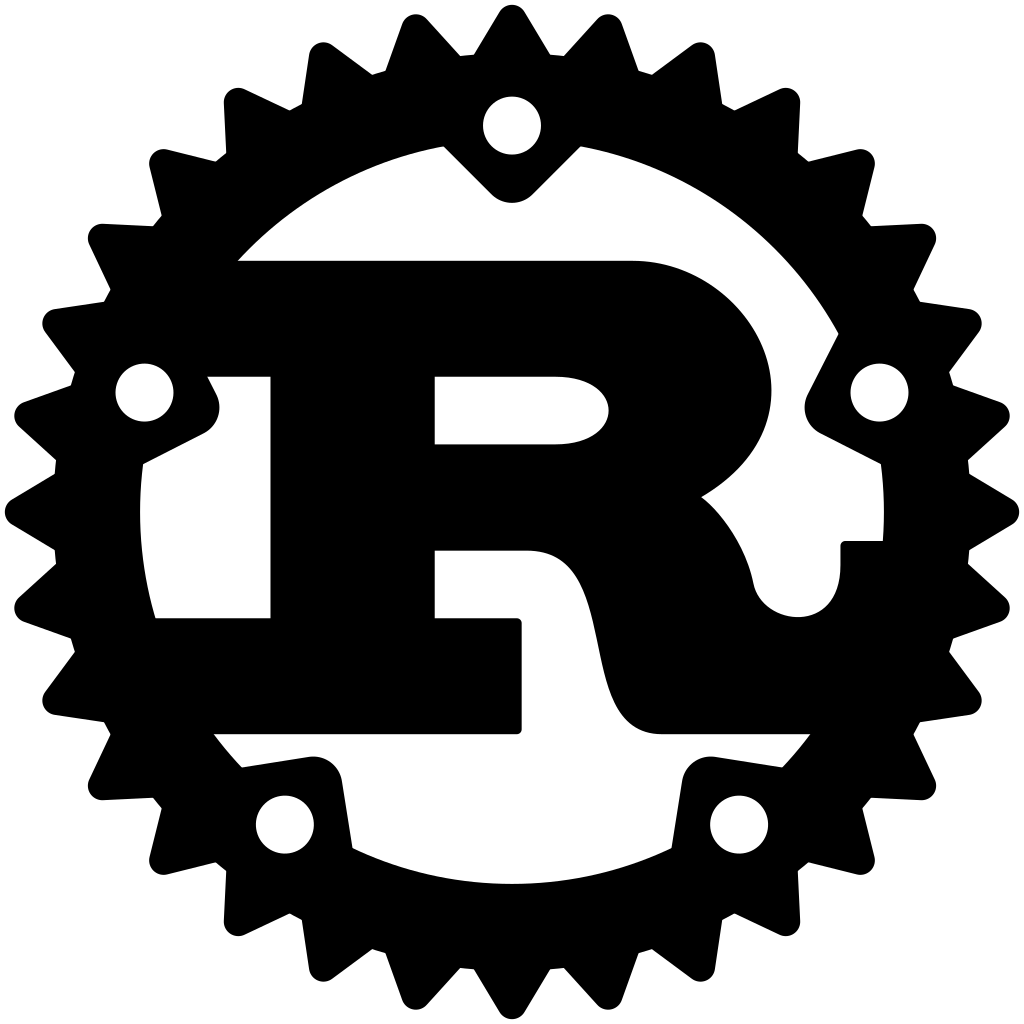
\includegraphics[width=\linewidth]{images/logos/rust.png} } %
  {\scriptsize \parbox[t]{\linewidth}{ Source: \url{https://foundation.rust-lang.org/policies/logo-policy-and-media-guide}} }
  \caption{Rust logo}
\end{wrapfigure}

In future releases, the Server implementation may and must be improved. \\ %
Replace any interpreted languages, such as \texttt{JavaScript} or \texttt{Python},
in the Server with a compiled/low-level programming language, such as \texttt{C},
\texttt{C++}, or \texttt{Rust}. Using these programming languages has two major advantages
over the existing implementation. First, because the program must be compiled to
produce the final executable, there is no need to distribute an archive or a
folder containing many files and then download and install all of the required
dependencies. The required dependencies must be available only on the machine performing
the compilation procedure, and if the program is compiled statically, all used libraries,
such as the OpenSSL library, are directly bundled inside the final executable,
at the expense of being larger than a dynamically linked program. Furthermore,
and this is critical, \cite{programming_languages_efficiency} reports that applications
that are implemented with a system programming language and are compiled directly
to machine code are significantly more efficient and demand fewer resources and energy
to accomplish the same result as an interpreted language. I would prefer \texttt{Rust}\footnote{\url{https://www.rust-lang.org}}
over the other two system languages because it guarantees memory safety and thread
safety, increasing overall reliability and productivity, even though it has a steep
learning curve at first, thanks to the various official tools, such as a package
manager and auto formatter. Although the development and effort required by a
compiled language is greater than that required by an interpreted language, the overall
benefits in this circumstance are too significant to be ignored. \\ %
Another area that needs to be enhanced is general error management and node administration,
since there is currently just a simple management of the two that heavily relies
on Kubernetes. Updated versions should improve error alerts to administrators as
well as possible recovery mechanisms. The latter can also be extended to use
various approaches based on the overall circumstances and deployment environment.
\\ %
Undoubtedly, many aspects of the Server could be improved but are not covered in
this section. However, because the project is completely FOSS compliant, users
can contribute and improve the code with ideas that I hadn't even considered
before.

\section{Closing Remarks}
\label{sec:conclusions_closing_remarks}

Adapting existing tools that are specifically developed for big and energy-hungry
environments to a more sustainable and resource-aware design while maintaining nearly
the same capabilities for a more green future for the computing industry is not only
feasible, but also necessary.


  \endgroup

  % Bibliography
  \addcontentsline{toc}{chapter}{Bibliography}
  % Alphabetical order of authors
  \bibliographystyle{plain}
  \bibliography{bibliography}


  % Attachments
  \titleformat{\chapter} {\normalfont\Huge\bfseries}{Appendix \thechapter}{1em}{}
  \appendix
  \chapter{Good Practices}
\label{cha:good_practices}

Many common software techniques, processes, and applications were used throughout
cluster implementation to improve overall code quality and to better and easily manage
the Git\footnote{\url{https://git-scm.com}} repository automatically. It would
be virtually impossible to list and explain them all in detail. Also, there are
several guides and publications available on them. Therefore, this attachment
will just briefly cover the two most well-known and widely used techniques that
have been used together, without going into much detail. \\ %
Finally, it is explained how the cluster implementation's final release archive
bundle is generated using a YAML configuration file and a POSIX script.

\section{DevOps}
\label{sec:good_practices_devops}

DevOps is a technique that integrates and automates Software Development (Dev) and
IT Operations (Ops). The combination of cultural philosophies, practices, and
tools improves an organization's capacity to provide applications and services
at high velocity: changing and enhancing products at a quicker rate than traditional
software development and infrastructure management procedures. Implementing a
DevOps paradigm for a project can result in significant benefits such as
increased speed, rapid delivery, reliability, scale, improved collaboration, and
security\cite{devops}. Figure \ref{fig:devops} depicts the cyclical collection of
DevOps phases. Depending on their primary goal, organizations might prioritize different
aspects of the DevOps paradigm.

DevOps is essential in modern software development and is intrinsically linked to
the Continuous Practices discussed in the next section.

\begin{figure}[htbp]
  \centering
  \def\stackalignment{r}\stackunder{ 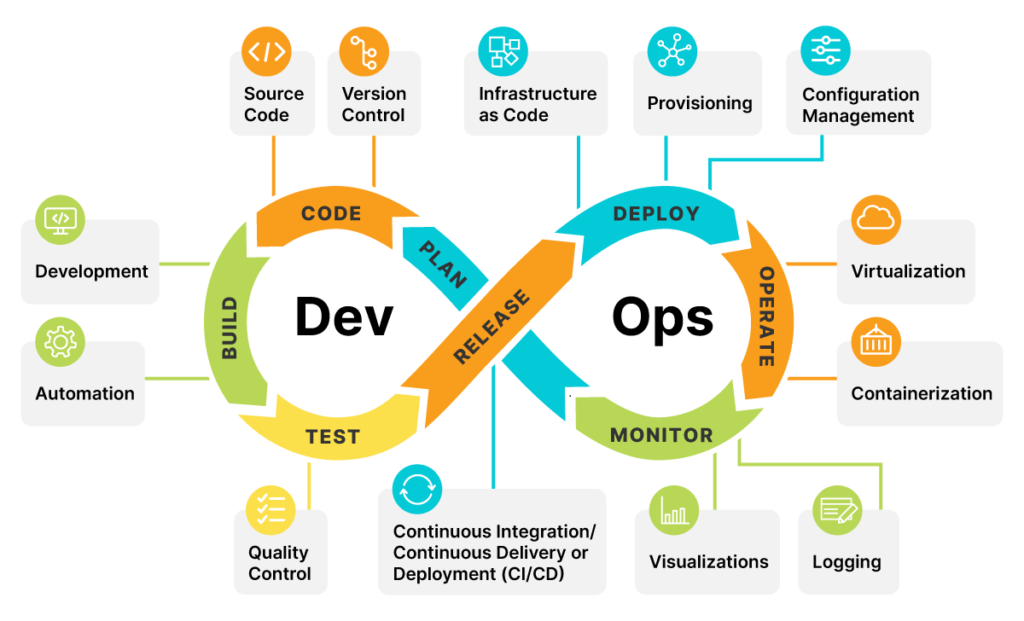
\includegraphics[width=.8\linewidth]{images/attachments/devops.png} } %
  {\scriptsize Source: \url{https://www.edureka.co/blog/what-is-devops} }
  \caption{Cyclical collection of DevOps phases}
  \label{fig:devops}
\end{figure}

\section{Continuous Practices}
\label{sec:continuous_practices}

Continuous Practices also referred to as Continuous Integration, Delivery, and Deployment,
are software development industry strategies that enable organizations to
release new features and products on a regular and consistent basis while
simultaneously keeping the code repository in a consistent state\cite{continuous_practices}.
When a new change is made to the code and pushed to the main repository, it is automatically
checked, compiled, and tested to guarantee code standards, consistency, and that
there are no potentially breaking changes in the prior application's behavior.
The relationship between the three Continuous Practices is depicted in figure
\ref{fig:continuous_practices}.

\begin{figure}[htbp]
  \centering
  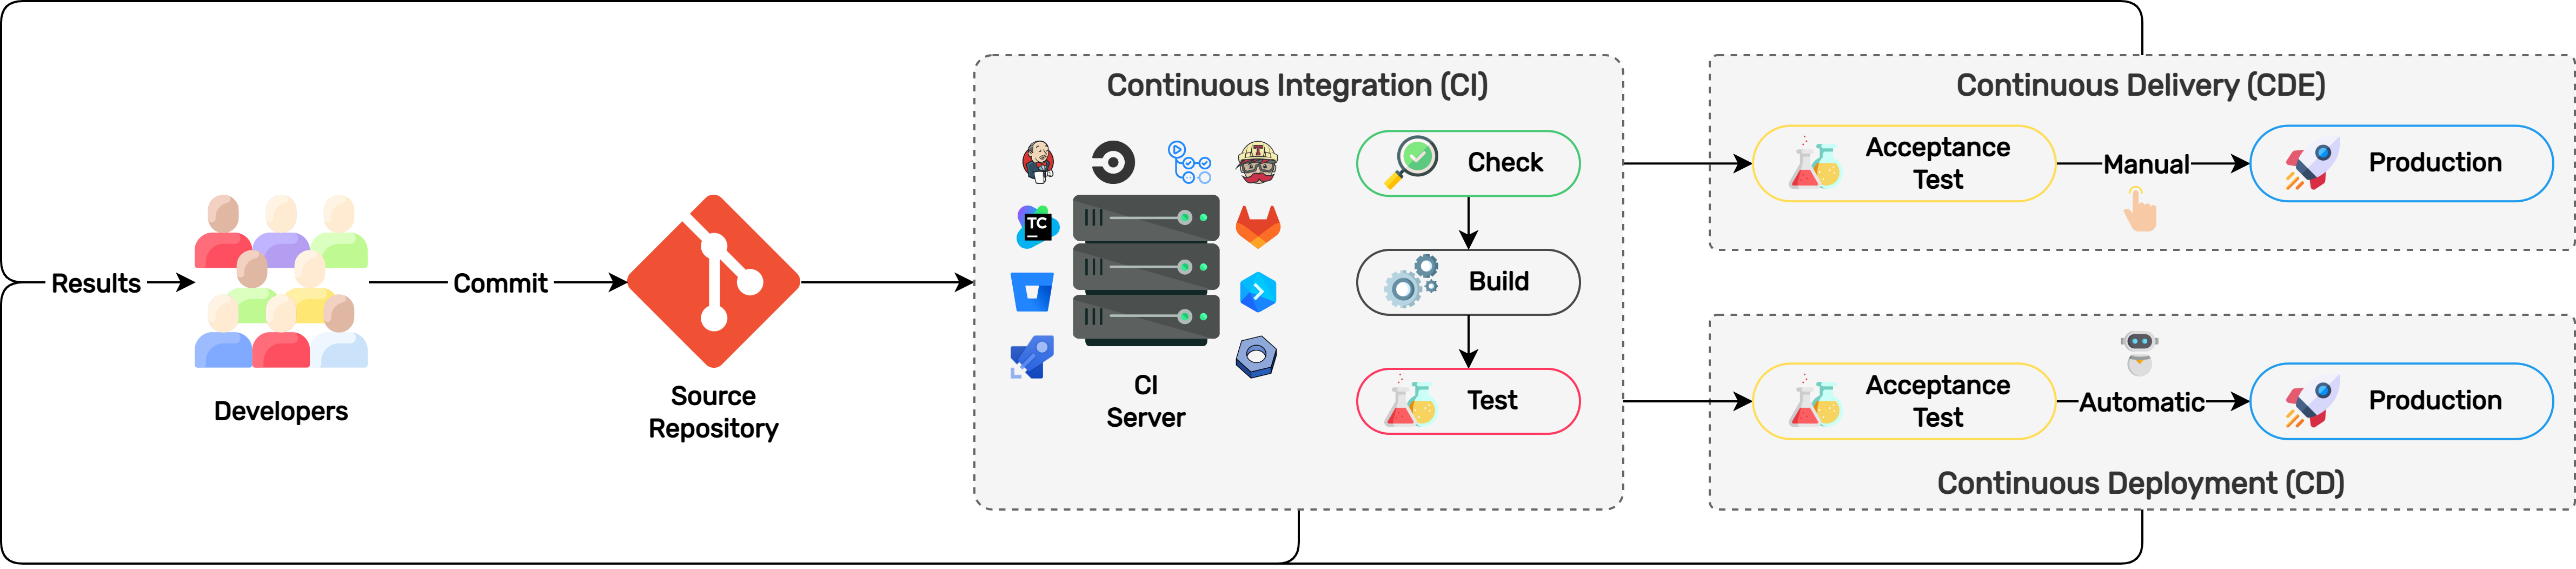
\includegraphics
  [width=.9\linewidth]{images/attachments/continuous_practices.png}
  \caption{Relationship between Continuous Integration, Delivery and Deployment}
  \label{fig:continuous_practices}
\end{figure}

Two automatic workflows to manage Continuous Practices on the source repository have
been implemented in the cluster implementation using GitHub Actions\footnote{\url{https://docs.github.com/actions}}.
The first workflow\footnote{\url{https://github.com/carlocorradini/reCluster/blob/main/.github/workflows/ci.yml}}
executes CI and CDE operations, while the second workflow\footnote{\url{https://github.com/carlocorradini/reCluster/blob/main/.github/workflows/codeql.yml}}
scans the code and generates security alerts if any known security vulnerabilities
are discovered. Furthermore, Dependabot\footnote{\url{https://github.com/dependabot/dependabot-core}}
has been added to keep all project dependencies up to date and to inform when a security
vulnerability is identified on a certain installed version. \\ %
Because of the use of Git Hooks\footnote{\url{https://git-scm.com/book/en/v2/Customizing-Git-Git-Hooks}},
a kind of local CI pipeline that examines every file before committing has also
been developed\footnote{\url{https://github.com/carlocorradini/reCluster/blob/main/.husky/pre-commit}}.
Because it may be skipped with a configuration flag, this procedure does not
substitute a true CI server. \\ %
The previously mentioned CI/CDE workflow fully automates the creation of a new
release\footnote{\url{https://github.com/carlocorradini/reCluster/releases}}. When
a new Git Tag\footnote{\url{https://git-scm.com/book/en/v2/Git-Basics-Tagging}} is
pushed to the main repository and the CI pipeline succeeds, the current cluster
implementation code is bundled (see section \ref{sec:good_practices_bundle}) and
released with the same name as the Git Tag. In the future, a CD pipeline will be
implemented that automatically produces a prerelease anytime a new change in the
code is made, ensuring that the newest nightly code is always available, even if
it is not as stable as a tagged release. \\ %
It should be noted that all prior implementations of Continuous Practices rely
on the GitHub platform. Yet, there are equivalent implementations for
practically every other coding platform.

\subsection{Continuous Integration}
\label{subsec:good_practices_continuous_practices_continuous_integration}

Continuous Integration (CI) is a well-established development process in the software
development industry in which team members regularly integrate and merge development
work (e.g., code). CI allows software organizations to have shorter and more
frequent release cycles, enhance software quality, and raise overall
productivity. This practice involves automated software checking, building and
testing\cite{continuous_practices}.

\subsection{Continuous Delivery}
\label{subsec:good_practices_continuous_practices_continuous_delivery}

Continuous Delivery (CDE) aims to ensure that an application is always ready for
production after passing automated tests and quality checks. CDE leverages a collection
of processes, such as CI and deployment automation, to deliver software automatically
to a production-like environment. This method has various advantages, including fewer
deployment risks, cheaper costs, and faster user feedback. Having a Continuous
Delivery approach necessitates a Continuous Integration process.\cite{continuous_practices}.

\subsection{Continuous Deployment}
\label{subsec:good_practices_continuous_practices_continuous_deployment}

Continuous Deployment (CD) deploys an application to production or customer environments
automatically and continuously. What distinguishes Continuous Deployment from
Continuous Delivery is the presence of a production environment (i.e., actual customers):
the purpose of Continuous Deployment practice is to automatically and consistently
deploy every update into the production environment. It's important to note that
CD practice implies CDE practice, but not the opposite. While the final
deployment in CDE is a manual process, there should be no manual steps in CD,
where changes are pushed to production as soon as developers commit them via a
deployment pipeline. \\ %
CDE is a pull-based approach in which an organization determines what and when
to deploy; CD is a push-based approach. In other words, CDE's scope excludes frequent
and automatic release, and CD is therefore a continuation of CDE. While CDE may be
applied to all kinds of systems and organizations, CD may only be appropriate
for particular types of organizations or systems\cite{continuous_practices}.

\section{Bundle}
\label{sec:good_practices_bundle}

To distribute a release of the cluster implementation, a mechanism that bundles all
required files and directories in a single archive file have been implemented.
The bundle is created automatically by the CDE workflow pipeline and uploaded on
GitHub with the name \texttt{recluster.tag.gz}. The archive file is composed of
a configuration file (see section \ref{subsec:good_practices_bundle_configuration})
that lists all necessary files and directories, and a POSIX script (see section
\ref{subsec:good_practices_bundle_script}) reads the configuration file and generates
the archive file, which may then be published. \\ %
It should be noted that the CDE pipeline is not required to build a bundle. The latter
enables organizations that do not wish to use the workflow to generate a bundle or
to locally test a cluster with a different implementation without involving any workflow.

\subsection{Configuration}
\label{subsec:good_practices_bundle_configuration}

The bundle configuration file, \texttt{bundle.config.yaml}, is written in \texttt{YAML}
format. \\ %
The attributes structure is a mapping that adheres to the development project's
tree hierarchy organization of files and directories\footnote{\url{https://github.com/carlocorradini/reCluster}}.
The key of an attribute is the file or directory name, and the value can be of
two types:
\begin{enumerate}
  \item \texttt{boolean}
    \newline
    The \texttt{true} value indicates that the file or directory should be copied
    (recursively), whereas the \texttt{false} value indicates that the file or directory
    should be ignored.
    \newline
    When the value is \texttt{true} and it is a directory, the included files
    and directories are copied in the order specified by the Git index and
    working tree\footnote{\url{https://git-scm.com/docs/git-ls-files}}.

  \item \texttt{mapping}
    \newline
    Applicable exclusively to a directory (parent), defines a mapping of files and
    directories that are contained in the parent directory.
    \newline
    A special metadata attribute, defined as \texttt{\_\_}, does not reflect a
    directory tree mapping and is instead employed by the script for specific
    operations and management that are applied to the current directory where
    the special attribute is located. At the moment, the only attribute that can
    be defined in the metadata is \texttt{run}, which provides an inline POSIX
    command. When generating the bundle file, all metadata attributes are
    examined and, if a \texttt{run} is identified, it is executed. It should be
    noted that the working directory for \texttt{run} is always the directory containing
    the metadata attribute. If the first two characters are \texttt{./}, the absolute
    path of the project's root directory is substituted. This facilitates the
    execution of scripts from various directories.
\end{enumerate}
Listing \ref{lst:bundle_config} displays the contents of the \texttt{bundle.config.yaml}\footnote{\url{https://github.com/carlocorradini/reCluster/blob/main/scripts/bundle.config.yaml}}
bundle configuration file. It is worth noting the use of the metadata attribute \texttt{\_\_}
in combination with the \texttt{run} attribute for executing applications and/or
programs that provide various outputs required for the release bundle.

\begin{lstlisting}[language=yaml, alsoletter={._-}, morekeywords={[2]{__, run, install.sh, LICENSE, README.md, configs, certs, k3s, k8s, autoscaler, loadbalancer, config.yaml, deployment.yaml, registry, node_exporter, recluster, ssh, dependencies, prometheus, distributions, alpine, arch, logo.png, iso, docs, scripts, certs.sh, configs.sh, configs.config.yaml, server, package.json, package-lock.json, build, prisma, schema.prisma, migrations}}, xleftmargin=\parindent, label={lst:bundle_config}, caption=Content of bundle configuration file]
  __:
    run: './scripts/inline.sh --in-file ./install.sh --overwrite'
  install.sh: true
  LICENSE: true
  README.md: true

  configs:
    README.md: true
    certs: true
    k3s: true
    k8s:
      README.md: true
      autoscaler: true
      loadbalancer:
        __:
          run: 'wget --output-document=deployment.yaml https://raw.githubusercontent.com/metallb
                  /metallb/v0.13.7/config/manifests/metallb-native.yaml'
        config.yaml: true
        deployment.yaml: true
        README.md: true
      registry: true
    node_exporter: true
    recluster: true
    ssh: true

  dependencies:
    __:
      run: './dependencies/dependencies.sh --sync-force'
    autoscaler: true
    k3s: true
    node_exporter: true
    prometheus: true

  distributions:
    alpine:
      __:
        run: './distributions/alpine/build.sh'
      README.md: true
      logo.png: true
      iso: true
    arch:
      __:
        run: './distributions/arch/build.sh'
      README.md: true
      logo.png: true
      iso: true

  docs: true

  scripts:
    __:
      run: './scripts/inline.sh --in-file ./certs.sh --overwrite && ./scripts/inline.sh --in-file
              ./configs.sh --overwrite'
    README.md: true
    certs.sh: true
    configs.sh: true
    configs.config.yaml: true

  server:
    __:
      run: 'npm run build:clean && npm run build'
    README.md: true
    package.json: true
    package-lock.json: true
    build: true
    prisma:
      schema.prisma: true
      migrations: true
\end{lstlisting}

\subsection{Script}
\label{subsec:good_practices_bundle_script}

To automate all bundle-related procedures, a POSIX script named \texttt{bundle.sh}\footnote{\url{https://github.com/carlocorradini/reCluster/blob/main/scripts/bundle.sh}}
is used. Its primary function is to read the bundle configuration file, read
metadata attributes, and generate a bundle archive file containing all files and
directories specified therein. \\ %
The script requires some \texttt{coreutils} package's utility programs and the
\texttt{yq} application to correctly handle \texttt{YAML} file and syntax. \\ %
application. \\ %
The script behavior of the bundle can be changed using parameter flags. The acceptable
setup settings are provided in the table below.

\begin{xltabular}
  {\textwidth} { >{\ttfamily}l | X | >{\ttfamily}c }

  \multicolumn{1}{ c |}{\large{\textbf{Name}}} &
  \multicolumn{1}{ c |}{\large{\textbf{Description}}} &
  \multicolumn{1}{ c }{\large{\textbf{Default Value}}} \\ \hhline{===}

  --config-file <FILE> & Path to the bundle configuration file (\texttt{<FILE>}).
  \newline
  Both relative and absolute paths are supported.
  \newline
  It should be noted that the configuration file name does not have to be \texttt{bundle.config.yaml},
  but may be any name and extension. The sole condition is that it must be in
  \texttt{YAML} format and that the attributes structure is respected. & bundle.config.yaml
  \\ \hline

  --out-file <FILE> & Name of the file path where the generated bundle archive file
  should be saved.
  \newline
  Absolute and relative paths are both supported.
  \newline
  By default, it is saved in the current working directory.
  \newline
  The extension name should always be \texttt{.tar.gz} to distinguish a compressed
  tar archive file. & bundle.tar.gz \\ \hline

  --skip-run & Skip all commands in the metadata attribute \texttt{run}. & false
  \\ \hline

  --log-level <LEVEL> & Logging level (\texttt{<LEVEL>}).
  \newline
  Attachment \ref{cha:logging} provides additional information regarding logging
  and logging levels.
  \newline
  The following logging levels are supported (listed in descending order of
  importance):
  \begin{itemize}[noitemsep]
    \item[\protect\icircled{\texttt{5}}] \texttt{fatal}

    \item[\protect\icircled{\texttt{4}}] \texttt{error}

    \item[\protect\icircled{\texttt{3}}] \texttt{warn}

    \item[\protect\icircled{\texttt{2}}] \texttt{info}

    \item[\protect\icircled{\texttt{1}}] \texttt{debug}
  \end{itemize}
  & info \\ \hline

  --help & Display a help message and terminate (successfully). & \\ \hline

  \caption{Bundle script parameters}
\end{xltabular}

To generate an archive bundle file, named \texttt{recluster.tar.gz}, that contains
all files and directories listed in the configuration file, just execute: \lstinline[language=shell,
alsoletter={.-}, morekeywords={[2]{bundle.sh}}, morekeywords={[3]{--out-file}}]{./bundle.sh --out-file "recluster.tar.gz"}
  \chapter{Corollary Projects}
\label{cha:corollary_projects}

During the development, I noticed that several portions of the code might be
turned into independent libraries and utility scripts that may be valuable to
other programmers as well as my single use-case scenario. Even though it is now external
to reCluster, this software is still an essential part of it, which is now open to
the entire community. \\ %
Shortly after the publication, I began receiving some feedback, contributions,
and, most importantly, appreciation in the form of GitHub stars\footnote{\url{https://docs.github.com/en/get-started/exploring-projects-on-github/saving-repositories-with-stars}}.
\\ %
% TODO Reference Philosophy and MIT
The three projects derived from the development of reCluster are briefly
illustrated and explained in the sections that follow. As stated in the Philosophy
section, everything is completely Open Source and available under the MIT
license.

\section{Node Exporter Installer}
\label{sec:corollary_projects_node_exporter_installer}

% TODO Node exporter reference
% TODO K3s reference
Available at \url{https://github.com/carlocorradini/node\_exporter\_installer} \\ %
Used while installing reCluster on a Node. \\ %
Node exporter does not provide any installation script and the default procedure
(see \url{https://github.com/prometheus/node_exporter#installation-and-usage})
is far from user-friendly and easily configurable. \\ %
Inspired by K3s \texttt{install.sh}\footnote{\url{https://github.com/k3s-io/k3s/blob/master/install.sh}}
script, Node exporter installer helps the user by automatically installing Node
exporter on the machine. Condensed in a single \texttt{install.sh} POSIX script,
it is easily configurable (see section
\ref{subsec:corollary_projects_node_exporter_installer_configuration}) and can be
downloaded and executed directly by \texttt{sh} (see example \ref{subsubsec:corollary_projects_node_exporter_installer_example_basic}).

\subsection{Configuration}
\label{subsec:corollary_projects_node_exporter_installer_configuration}

Node exporter installer accepts environment variables only as configuration parameters.
This is done to avoid any potential conflict with the default behavior of Node
exporter, which employs argument flags. See
\url{https://github.com/prometheus/node\_exporter\#collectors} for a
comprehensive list of Node exporter configuration parameters. \\ %
The configuration settings allowed by Node exporter installer are shown in the
table below.

\begin{xltabular}
  {\textwidth} { >{\ttfamily}l | X | >{\ttfamily}c }

  \multicolumn{1}{ c |}{\large{\textbf{Name}}} &
  \multicolumn{1}{ c |}{\large{\textbf{Description}}} &
  \multicolumn{1}{ c }{\large{\textbf{Default Value}}} \\ \hline \hline

  INSTALL\_NODE\_EXPORTER\_SKIP\_DOWNLOAD & Skip downloading Node exporter.
  \newline
  A local executable binary must already exist at \texttt{<BIN\_DIR>/node\_exporter}
  \newline
  Useful in an Air-Gapped environment. % TODO Air-Gap environment reference
  & false \\ \hline

  INSTALL\_NODE\_EXPORTER\_FORCE\_RESTART & Force restarting Node exporter
  service. & false \\ \hline

  INSTALL\_NODE\_EXPORTER\_SKIP\_ENABLE & Do not enable Node exporter service at
  startup. & false \\ \hline

  INSTALL\_NODE\_EXPORTER\_SKIP\_START & Do not start Node exporter service. & false
  \\ \hline

  INSTALL\_NODE\_EXPORTER\_SKIP\_FIREWALL & Do not apply any firewall rules.
  \newline
  Supported firewalls are: \texttt{iptables}\footnote{\url{https://www.netfilter.org/projects/iptables}},
  \texttt{firewalld}\footnote{\url{https://firewalld.org}} and \texttt{UFW}\footnote{\url{https://wiki.ubuntu.com/UncomplicatedFirewall}}.
  & false \\ \hline

  INSTALL\_NODE\_EXPORTER\_SKIP\_SELINUX & Do not change \texttt{SELinux\footnote{\url{https://selinuxproject.org}}}
  context for Node exporter binary. & false \\ \hline

  INSTALL\_NODE\_EXPORTER\_VERSION & Node exporter version to download. & latest
  \\ \hline

  INSTALL\_NODE\_EXPORTER\_BIN\_DIR & Directory where to install Node exporter binary
  and uninstall script. & \makecell[Xt]{\centering{/usr/local/bin \\ or \\ /opt/bin}}
  \\ \hline

  INSTALL\_NODE\_EXPORTER\_SYSTEMD\_DIR & Directory where to install Systemd service
  files. & /etc/systemd/system \\ \hline

  INSTALL\_NODE\_EXPORTER\_EXEC & Node exporter configuration flags. & \\

  \caption{Node exporter installer configuration parameters}
\end{xltabular}

\subsection{Example}
\label{subsec:corollary_projects_node_exporter_installer_example}

This section shows some examples of how to use Node exporter installer. In both,
we use \texttt{curl} (a command-line tool for getting or sending data using URL
syntax\cite{curl}) to download the script from
\url{https://raw.githubusercontent.com/carlocorradini/node_exporter_installer/main/install.sh}
and pipe (redirect the output of a program to the input of another program) the
result to \texttt{sh} (UNIX shell command-line interpreter\footnote{\url{https://wikipedia.org/wiki/Unix_shell}})
for execution.

\subsubsection{Basic}
\label{subsubsec:corollary_projects_node_exporter_installer_example_basic}

Install Node exporter using the default configuration parameters for both
installer and binary.

\begin{lstlisting}[language=sh, morekeywords={curl, sh}, morestring={[s]{.sh}}, xleftmargin=\parindent, caption=Basic installation with default configuration parameters]
  curl \
    --silent \      # Do not show progress meter or error messages
    --show-error \  # Show an error message if it fails
    --fail \        # Fail fast with no output at all on server errors
    --location \    # If the requested resource has moved, redo the request to the new location
    "https://raw.githubusercontent.com/carlocorradini/node_exporter_installer/main/install.sh" \
    | sh -
\end{lstlisting}

\subsubsection{Advanced}
\label{subsubsec:corollary_projects_node_exporter_installer_example_advanced}

Install Node exporter v1.5.0 without starting the service automatically. Disable
all default collectors, leaving only CPU and memory statistics enabled.

\begin{lstlisting}[language=sh, morekeywords={curl, sh}, xleftmargin=\parindent, caption=Advanced installation with custom configuration parameters]
  curl \
    ... \
    | INSTALL_NODE_EXPORTER_VERSION="v1.5.0" \   # Download and install Node exporter v1.5.0
      INSTALL_NODE_EXPORTER_SKIP_START="true" \  # Do not start Node exporter service
      sh - \
        --collector.disable-defaults \             # Disable default collectors
        --collector.cpu \                          # Expose CPU statistics
        --collector.meminfo                        # Expose memory statistics
\end{lstlisting}

\section{Inline}
\label{sec:corollary_projects_inline}

% TODO Bundle reference
Available at \url{https://github.com/carlocorradini/inline} \\ %
Used while generating the final release bundle for distribution. \\ %
It is useful to be able to split a large script into many files to make it easier
to work with while still being able to distribute it as a single script. This
program reads an input file and produces an output file with all of the sources
inlined. \\ %
The source command, \texttt{.\ <FILE>} for POSIX shells or \texttt{source <FILE>}
for non-POSIX shells (e.g. Bash\footnote{\url{https://www.gnu.org/software/bash}}),
read, and executes commands from the file specified in the current shell
environment. It is useful to load functions, variables, and configuration files into
the current shell context\cite{source}. \\ %
Inline is a static tool that does not execute the input script. As a result, it
cannot determine the value of a variable dynamically if it is used inside the
source command path (i.e. \texttt{source "\$DIR/path/to/script/sh"}). To avoid
this, inline requires a hint on where to find the specified file.

\subsection{Features}
\label{subsec:corollary_projects_inline_features}

Many helpful features of Inline are described below.

\begin{itemize}
  \item POSIX standard-compliant.

  \item Sourcing with quotes, spaces, and more.

  \item Sourcing from global variable \texttt{\$PATH}.

  \item Sourcing from \texttt{ShellCheck} (a shell script static analysis tool\footnote{\url{https://www.shellcheck.net}})
    source directive\footnote{\url{https://www.shellcheck.net/wiki/Directive}}.
    \newline
    This is considered a hint to Inline and is used only if the source path is invalid.
    \newline
    \begin{lstlisting}[language=sh, morekeywords={., source}, numbers=none, aboveskip=0pt, belowskip=0pt, abovecaptionskip=0pt, belowcaptionskip=0pt]
      # shellcheck source=path/to/script.sh
      . "$DIR/path/to/script.sh"

      # shellcheck source=path/to/script.sh
      source "$DIR/path/to/script.sh"
    \end{lstlisting}

  \item Recursive sources. If a sourced file contains additional source commands,
    they are also inlined and included in the final output script.
    \newline
    It should be noted that these can cause infinite recursion.

  \item Recursion detection. To avoid infinite recursion, an exception is thrown
    if a file is sourced multiple times. This is accomplished through the use of
    an internal cache that saves the absolute path to each sourced file. If the path
    to a script file in a source command is already in the cache, a recursion is
    detected.

  \item Shebang removal in sourced files.
    \newline
    A shebang is the character sequence consisting of the characters number sign
    and exclamation mark (\texttt{\#!}) at the beginning of a script. In a Unix-like
    operating system, when a text file with a shebang is used as if it is an
    executable, the program loader executes the specified interpreter program,
    passing as an argument the path that was initially used when attempting to
    run the script, so that the program can use the file as input data\cite{shebang}
    \newline
    The shell interpreter only allows one shebang per script. As a result, the
    shebang is only allowed in the input script file, while it is automatically removed
    in all sourced script files.

  \item Avoid inlining a certain source file. If the inline skip comment
    directive (\texttt{\# inline skip}) is present before a source command, the
    latter is ignored and not inlined. As a consequence, the final output script
    includes the original command, unaltered and unaligned.
    \newline
    It is worth noting that the skip directive also works with ShellCheck. The sole
    requirement is that there are no blank lines between the directives and the source
    command.
    \newline
    \begin{lstlisting}[language=sh, morekeywords={., source}, numbers=none, aboveskip=0pt, belowskip=0pt, abovecaptionskip=0pt, belowcaptionskip=0pt]
    # inline skip
    # shellcheck source=path/to/script.sh
    . "$DIR/path/to/script.sh"

    # shellcheck source=path/to/script.sh
    # inline skip
    source "$DIR/path/to/script.sh"
  \end{lstlisting}
\end{itemize}

\subsection{Configuration}
\label{subsec:corollary_projects_inline_configuration}

Inline's behavior is easily customizable by using argument flags, which begin with
a double dash followed by the property name and an optional value (\texttt{--NAME
[VALUE]}). \\ %
The accepted configuration parameters are listed in the table below.

\begin{xltabular}
  {\textwidth} { >{\ttfamily}l | X | >{\ttfamily}c }

  \multicolumn{1}{ c |}{\large{\textbf{Name}}} &
  \multicolumn{1}{ c |}{\large{\textbf{Description}}} &
  \multicolumn{1}{ c }{\large{\textbf{Default Value}}} \\ \hline \hline

  --in-file <FILE> & Input script file (\texttt{<FILE>}).
  \newline
  If the file does not exist, an error is thrown. & \\ \hline

  --out-file <FILE> & Output script file (\texttt{<FILE>}).
  \newline
  If a file with the same name and path already exists, an error is thrown.
  Unless the \texttt{--overwrite} argument is given, the latter is always true (see
  option below).
  \newline
  If no value is specified, the name of the output file is determined by
  examining the original input file. The first portion is the original name,
  followed by a \texttt{.inlined} string, and finally, if present, the extension
  (usually \texttt{.sh}). & <NAME>.inlined[EXTENSION] \\ \hline

  --overwrite & Replace the input file.
  \newline
  The inlined result replaces the original file content. This is the same as
  setting the output file's value as the original input file, except that the existence
  check is bypassed (see option above). & false \\ \hline

  --log-level <LEVEL> & Logging level (\texttt{<LEVEL>}).
  \newline
  A level is chosen from the list below (in descending order of priority), with
  the expectation that lower levels are ignored in favor of the higher ones.
  \begin{itemize}[noitemsep]
    \item \texttt{fatal}
      \newline
      Extremely serious error events that most likely cause the program to
      terminate.

    \item \texttt{warn}
      \newline
      Potentially dangerous conditions.

    \item \texttt{info}
      \newline
      Informational messages that emphasize the application's progress at a
      coarse-grained level.

    \item \texttt{debug}
      \newline
      Fine-grained informative events are most helpful when debugging an
      application.

    \item \texttt{silent}
      \newline
      Disable logging.
  \end{itemize}
  & info \\ \hline

  --disable-color & Disable terminal colors (enabled by default). & false \\ \hline

  --help & Display a help message and terminate (successfully). & \\

  \caption{Inline configuration parameters}
\end{xltabular}

\subsection{Example}
\label{subsec:corollary_projects_inline_example}

This section provides an example of how Inline works and how it may be used. \\ %
There are two script files, both of which begin with a shebang. There is a print
command in the first file, \texttt{hello.sh}, that outputs \texttt{Hello} and an
empty space, followed by a source command that includes the script file \texttt{world.sh}.
The format of the second file, \texttt{world.sh}, is the same as the first, except
that the print command outputs \texttt{World!} and the newline character (\texttt{\char`\\n}),
and there are no source commands. \\ %
The following two listings show the contents of the two files:

\noindent
\hspace{.775\parindent}
\begin{minipage}[t]{.45\textwidth}
  \begin{lstlisting}[language=sh, morekeywords={., printf}, caption=Input script \texttt{hello.sh}]
    #!/usr/bin/env sh

    printf "Hello "

    . "world.sh"
  \end{lstlisting}
\end{minipage}
\hfill
\begin{minipage}[t]{.45\textwidth}
  \begin{lstlisting}[language=sh, morekeywords={., printf}, caption=Sourced script \texttt{world.sh}]
    #!/usr/bin/env sh

    printf "World!\n"
  \end{lstlisting}
\end{minipage}

The goal is to inline the script file \texttt{hello.sh} and produce an output
file that has no source commands. When the command %
\lstinline[language=sh, basicstyle=\ttfamily, deletekeywords={in}, alsoletter={.},
morekeywords={inline.sh}]{./inline.sh --in-file "hello.sh"} %
is executed, the following result is obtained:

\begin{lstlisting}[language=sh, morekeywords={., printf}, xleftmargin=\parindent, caption=Inlined script \texttt{hello.inlined.sh}]
  #!/usr/bin/env sh

  printf "Hello "

  # . "world.sh"

  printf "World!\n"
\end{lstlisting}

Note the unique shebang as well as the source command that has been commented out
with the symbol \texttt{\#}. Furthermore, because no \texttt{--out-file} option is
used, the final output file is named \texttt{hello.inlined.sh}, which does not
override the original input file.

\section{GraphQL Auth Directive}
\label{sec:corollary_projects_graphql_auth_diretive}

% TODO GraphQL reference
% TODO Node.js reference
Available at \url{https://github.com/carlocorradini/graphql-auth-directive} \\ %
Used in the \texttt{GraphQL} API. \\ %
A custom \texttt{GraphQL} directive that protects resources from unauthenticated
and unauthorized access in high-security contexts. It is available in all major \texttt{Node.js}
registries as \texttt{graphql-auth-directive}. \\ %
A directive is an identifier preceded by a \texttt{@} character, optionally followed
by a list of named arguments, which can appear after almost any form of syntax
in the \texttt{GraphQL} query or schema languages\cite{graphql_directive}. \\ %
The \texttt{GraphQL} context holds all important information about the current request.
A \texttt{GraphQL} context is an object that is shared by all resolvers in a given
execution. It helps store data such as authentication information, the current user,
database connections, data sources, and other information required to operate
the business logic\cite{graphql_context}. It is important to note that the
context does not have to follow a predefined structure; rather, it is highly
flexible to the user's implementation.

\subsection{Configuration}
\label{subsec:corollary_projects_graphql_auth_diretive_configuration}

Before applying the directive to the \texttt{GraphQL} schema, it must be built/configured.
The library exposes a utility function called \texttt{buildAuthDirective} that accepts
a configuration object with the values provided in the table below and returns the
type definition (see section
\ref{subsec:corollary_projects_graphql_auth_diretive_type_definition}) as well as
a transformer function that applies the auth logic to the executable \texttt{GraphQL}
schema.

\begin{xltabular}
  {\textwidth} { >{\ttfamily}l | X | >{\ttfamily}c }

  \multicolumn{1}{ c |}{\large{\textbf{Name}}} &
  \multicolumn{1}{ c |}{\large{\textbf{Description}}} &
  \multicolumn{1}{ c }{\large{\textbf{Default Value}}} \\ \hline \hline

  name & Directive name.
  \newline
  If a name different from the default is specified, it must be reflected in the
  schema where the directive is used, otherwise, an error is thrown. & auth \\
  \hline

  auth & A function or class that handles authentication and authorization.
  \newline
  The current context (which contains information about the current request) and
  the roles and permissions required by the requested resource must be accepted
  as arguments by the implementation. If access to the requested resource is granted,
  the boolean value \texttt{true} is returned; otherwise, \texttt{false} is
  returned if access is denied.
  \newline
  A default basic auth function is already implemented and checks for the existence
  of an authorized applicant and that its roles and permissions overlap with those
  of the requested resource. & \\ \hline

  authMode & Auth mode if access is not granted.
  \newline
  Methodology for informing the requestor that access to the resource has been
  denied. It is often desirable to hide the important information that the request
  is failing due to an auth check and instead deliver an error/informational response
  stating that the requested resource simply does not exist.
  \newline
  The first mode, \texttt{ERROR}, throws an authentication or authorization error
  (see below), whereas the second mode, \texttt{NULL}, returns the value \texttt{null}
  (empty). & ERROR \\ \hline

  roles & Roles configuration.
  \newline
  An object with two properties:
  \begin{itemize}
    \item \texttt{enumName}
      \newline
      Defines the array type, which is by default a \texttt{String}.
      \newline
      It is standard practice in \texttt{GraphQL} and in programming languages
      to map a set of values to an enum. An enumeration type is a special kind of
      scalar that is restricted to a particular set of allowed values\cite{graphql_enum}.
      \newline
      This option restricts the allowed values of roles to a specific set rather
      than a general string.

    \item \texttt{default}
      \newline
      Roles that are required by default.
      \newline
      No roles are required by default. As a result, access to a protected resource
      can only be provided with authentication. Overriding this option enables
      authorization by default, requiring the requestor to have at least one matching
      role.
  \end{itemize}
  & \makecell[Xt]{\centering{enumName: String \\ default: []}} \\ \hline

  permissions & Permissions configuration.
  \newline
  An object with the same properties as roles configuration (see above). & \makecell[Xt]{\centering{enumName: String \\ default: []}}
  \\ \hline

  authenticationError & Authentication error class. The error is thrown if there
  is no authenticated requestor in the current context. By default, a generic error
  is thrown. The class must extend the \texttt{Error} class. &
  AuthenticationError \\ \hline

  authorizationError & Authorization error class. The error is thrown if the
  roles and/or permissions of the requestor do not overlap with those of the
  requested resource. By default, a generic error is thrown. The class must extend
  the \texttt{Error} class. & AuthorizationError \\ \hline

  container & Dependency Injection Container.
  \newline
  Dependency injection is a design pattern that shifts the responsibility of resolving
  dependencies to a dedicated dependency injector that knows which dependent objects
  to inject into application code\cite{dependency_injection}.
  \newline
  It should be noted that dependency injection is only available if \texttt{auth}
  is a class type. & IOCContainer \\

  \caption{GraphQL auth directive configuration parameters}
\end{xltabular}

\subsection{Type Definition}
\label{subsec:corollary_projects_graphql_auth_diretive_type_definition}

% TODO GraphQL reference
GraphQL has its language for writing GraphQL Schemas: the GraphQL Schema Definition
Language (SDL). SDL is incredibly powerful and expressive while being simple and
intuitive to use. The syntax is well-defined and is included in the official GraphQL
specification\footnote{\url{https://spec.graphql.org}}. Schema Definitions are
also known as IDL (Interface Definition Language) or SDL (Schema Definition Language)\cite{graphql_sdl}.
\\ %
The Type Definition of the GraphQL auth directive generated with default settings
is shown below:

\begin{lstlisting}[language=graphql, xleftmargin=\parindent, caption=GraphQL auth directive Type Definition]
  """
  Protect the resource from unauthenticated and unauthorized access.
  """
  directive @auth(
    """
    Allowed roles to access the resource.
    """
    roles: [String!]! = []
    """
    Allowed permissions to access the resource.
    """
    permissions: [String!]! = []
  ) on FIELD | FIELD_DEFINITION | OBJECT
\end{lstlisting}

The above definition must be available in every \texttt{GraphQL} schema that utilizes
the directive, otherwise an error is thrown during the server bootstrap
operation. \\ %
As stated in section
\ref{subsec:corollary_projects_graphql_auth_diretive_configuration}, the definition
is generated dynamically by a set of configuration options or their default value.
The name (\texttt{@auth}), \texttt{roles} and \texttt{permissions} type (non-nullable
\texttt{String} array), and default value (an empty array \texttt{[]}) are
easily distinguishable.

\subsection{Example}
\label{subsec:corollary_projects_graphql_auth_diretive_example}

Consider a \texttt{GraphQL} backend application that requires authentication and
authorization. The sections of the \texttt{GraphQL} schema where the auth
directive is used, as well as the enums that compose the different roles and permissions
mappings are listed below:

\begin{lstlisting}[language=graphql, xleftmargin=\parindent, caption=\texttt{GraphQL} schema with auth directive and mappings]
  enum Role {
    ADMIN
    SIMPLE
  }

  enum Permission {
    VIEW
    EDIT
  }

  directive @auth(
    roles: [Role!]! = []
    permissions: [Permission!]! = []
  ) on FIELD | FIELD_DEFINITION | OBJECT

  type Query {
    unprotected: String!
    protected(arg: Boolean): Int! @auth
    secret: Float! @auth(roles: [ADMIN], permissions: [VIEW])
  }
\end{lstlisting}

The available roles are represented by the enum \texttt{Role}: \texttt{ADMIN} for
administrators and \texttt{BASIC} for simple users. The supported permissions are
represented by the enum \texttt{Permission}: \texttt{VIEW} to allow resource
visualization and \texttt{EDIT} to allow resource modification. \\ %
The definition of \texttt{@auth} directive accepts as roles an array of \texttt{Role}
whose default value is empty and as permissions an array of \texttt{Permission}
whose default value is empty. Notice the difference from the default type definition
shown in section \ref{subsec:corollary_projects_graphql_auth_diretive_type_definition}.
\\ %
Three queries are supported:
\begin{enumerate}
  \item \lstinline[language=graphql, basicstyle=\ttfamily]{unprotected: String!}
    \newline
    \texttt{unprotected} does not accept any arguments and returns a non-nullable
    string. Does not require any authentication or authorization. As a result,
    it may be called by anyone.

  \item \lstinline[language=graphql, basicstyle=\ttfamily]{protected(arg: Boolean): Int! @auth}
    \newline
    \texttt{unprotected} accepts a boolean optional parameter named \texttt{arg}
    and returns a non-nullable integer number. Because no roles or permissions are
    specified in the directive, it requires only authentication but no
    authorization. As a consequence, everyone who has been authenticated is
    allowed to call this query.

  \item \lstinline[language=graphql, basicstyle=\ttfamily]{secret: Float! @auth(roles: [ADMIN], permissions: [VIEW])}
    \newline
    The most secure of the three, \texttt{secret}, does not take any parameters and
    returns a non-nullable float integer. The caller must have an admin role
    with view permission to use this query. As a consequence, the query is
    secured by both authentication and authorization, resulting in higher requirements
    to perform the desired action on the resource.
\end{enumerate}
  \chapter{Upstream Contributions}
\label{cha:upstream_contributions}

% TODO Contributions to other OSS software
% TODO Complex project development recognized pieces of the project useful to external parties

\section{Autoscaler}
\label{sec:upstream_contributions_autoscaler}

\url{https://github.com/kubernetes/autoscaler}

\subsection{Cluster Autoscaler Segmentation Violation}
\label{subsec:upstream_contributions_autoscaler_cluster_autoscaler_segmentation_violation}

\url{https://github.com/kubernetes/autoscaler/issues/5378}

\section{Prisma}
\label{sec:upstream_contributions_prisma}

\url{https://github.com/prisma/prisma}

\subsection{OpenSSL 3.0 In Alpine Linux 3.17}
\label{subsec:upstream_contributions_prisma_openssl_in_alpine_linux}

\url{https://github.com/prisma/prisma/issues/16553}

\section{ShellCheck}
\label{sec:upstream_contributions_shellcheck}

\url{https://github.com/gunar/shellcheck}

\subsection{Rewrite}
\label{subsec:upstream_contributions_shellcheck_rewrite}

\url{https://github.com/gunar/shellcheck/pull/34}

\section{TypeGraphQL}
\label{sec:upstream_contributions_typegraphql}

\url{https://github.com/MichalLytek/type-graphql}

\subsection{Maintainability Improvements}
\label{subsec:upstream_contributions_typegraphql_maintainability_improvements}

\url{https://github.com/MichalLytek/type-graphql/pull/1400}

\subsection{Postinstall Script}
\label{subsec:upstream_contributions_typegraphql_postinstall_script}

\url{https://github.com/MichalLytek/type-graphql/pull/1363}

\section{CSpell}
\label{sec:upstream_contributions_cspell}

\subsection{Shell Dictionary}
\label{subsec:upstream_contributions_cspell_shell_dictionary}

\url{https://github.com/streetsidesoftware/cspell-dicts/pull/1635}

\subsection{K8s Dictionary}
\label{subsec:upstream_contributions_cspell_k8s_dictionary}

\url{https://github.com/streetsidesoftware/cspell-dicts/pull/1704}

\section{VS Code Icons}
\label{sec:upstream_contributions_vscode_icons}

\subsection{ShellCheck}
\label{subsec:upstream_contributions_vscode_icons_shellcheck}

\url{https://github.com/vscode-icons/vscode-icons/pull/3174}
  \chapter{Logging}
\label{cha:logging}

Logging\footnote{\url{https://wikipedia.org/wiki/Logging_(computing)}} is the process
of preserving a record of events that occur in a computer system, such as issues,
errors, or just information on current operations. These events might happen in the
operating system or other applications. For each such event, a message or log entry
is recorded. These log messages may subsequently be used to monitor and
understand the system's operation, troubleshoot problems, or during an audit. Logging
is very crucial in multi-user applications to provide a centralized view of the system's
functionality. \\ %
It is critical in the architecture implementation to log the numerous operations
that occur in each component of the cluster. The latter not only assists in
understanding how the general architecture performs and its status, but also the
potential causes of an incident. During the cluster's development, if any components
failed or did not behave as they should (e.g., no autonomous upscaling or
downscaling), monitoring and analyzing the numerous log files created was the
only method to solve the problems and understanding what and why happened. Furthermore,
a logging system is available for the multitude of utility scripts and
applications that are not directly employed with the cluster but rather during
its general development. \\ %
Log interpretation is a challenging process. Log management system collects data
from a variety of sources with varying forms, purposes, and granularities.
Maintaining defined log levels helps give each entry meaning and better
understand the significance of the related log message\cite{logging_levels}.
Section \ref{sec:logging_levels} describes common logging levels that are also
employed in cluster development and implementation.

\section{Levels}
\label{sec:logging_levels}

A log level is a piece of information that indicates the importance of a log message.
It is a basic yet effective method of identifying log events from one another. Furthermore,
it is utilized to filter crucial information regarding the system state to only
those that are solely informational\cite{logging_levels}. \\ %
During the initialization phase, a level is chosen from the list below (sorted in
descending order of importance), with the expectation that the lower levels are ignored
in favor of the higher ones.

\begin{enumerate}
  \item[\protect\icircled{\texttt{7}}] \texttt{SILENT}
    \newline
    The highest possible logging level is meant to completely disable logging.

  \item[\protect\icircled{\texttt{6}}] \texttt{FATAL}
    \newline
    The system experienced a very severe error, which caused the system to abort.

  \item[\protect\icircled{\texttt{5}}] \texttt{ERROR}
    \newline
    Employed when the system encounters a problem that prevents one or more operations
    from functioning properly but allows it to continue operating.

  \item[\protect\icircled{\texttt{4}}] \texttt{WARN}
    \newline
    Designates potentially dangerous conditions that do not cause the system to crash.

  \item[\protect\icircled{\texttt{3}}] \texttt{INFO}
    \newline
    The standard log level indicates informational messages about the progress at
    a coarse-grained level. The information reported using the \texttt{INFO} log
    level should be strictly informative, without the need for any essential
    information to be lost.

  \item[\protect\icircled{\texttt{2}}] \texttt{DEBUG}
    \newline
    Used for information that may be required for diagnosing and debugging issues,
    or for running in a test environment to ensure that everything is working
    properly.

  \item[\protect\icircled{\texttt{1}}] \texttt{TRACE}
    \newline
    The most fine-grained level of information is only employed in rare circumstances
    where full visibility of what is occurring is required. \texttt{TRACE}'s logging
    level is quite verbose.
\end{enumerate}

Table \ref{tbl:logging_levels}, shows the correlation between the logging level and
the related logging message. The default logging level in various
implementations is often set to \texttt{INFO} level.

\begin{xltabular}
  {\textwidth} { >{\ttfamily}c | >{\large\ttfamily}c | >{\large\ttfamily}c | >{\large\ttfamily}c | >{\large\ttfamily}c | >{\large\ttfamily}c | >{\large\ttfamily}c }

  \multicolumn{1}{
  c
  |}{\backslashbox{\large{\textbf{Logging Level}}}{\large{\textbf{Logging Message}}}}
  & FATAL & ERROR & WARN & INFO & DEBUG & TRACE \\ \hhline{=======}

  \protect\icircled{\texttt{7}} SILENT & \cellcolor{bulmaRed}\hphantom{......} &
  \cellcolor{bulmaRed}\hphantom{......} & \cellcolor{bulmaRed}\hphantom{......}
  & \cellcolor{bulmaRed}\hphantom{......} & \cellcolor{bulmaRed}\hphantom{......}
  &\cellcolor{bulmaRed}\hphantom{......} \\ \hline

  \protect\icircled{\texttt{6}} FATAL\leavevmode\hphantom{.} & \cellcolor{bulmaGreen}
  & \cellcolor{bulmaRed} & \cellcolor{bulmaRed} & \cellcolor{bulmaRed} &
  \cellcolor{bulmaRed} & \cellcolor{bulmaRed} \\ \hline

  \protect\icircled{\texttt{5}} ERROR\leavevmode\hphantom{.} & \cellcolor{bulmaGreen}
  & \cellcolor{bulmaGreen} & \cellcolor{bulmaRed} & \cellcolor{bulmaRed} & \cellcolor{bulmaRed}
  & \cellcolor{bulmaRed} \\ \hline

  \protect\icircled{\texttt{4}} WARN\leavevmode\hphantom{..} & \cellcolor{bulmaGreen}
  & \cellcolor{bulmaGreen} & \cellcolor{bulmaGreen} & \cellcolor{bulmaRed} &
  \cellcolor{bulmaRed} & \cellcolor{bulmaRed}\\ \hline

  \protect\icircled{\texttt{3}} INFO\leavevmode\hphantom{..} & \cellcolor{bulmaGreen}
  & \cellcolor{bulmaGreen} & \cellcolor{bulmaGreen} & \cellcolor{bulmaGreen} &
  \cellcolor{bulmaRed} & \cellcolor{bulmaRed} \\ \hline

  \protect\icircled{\texttt{2}} DEBUG\leavevmode\hphantom{.} & \cellcolor{bulmaGreen}
  & \cellcolor{bulmaGreen} & \cellcolor{bulmaGreen} & \cellcolor{bulmaGreen} & \cellcolor{bulmaGreen}
  & \cellcolor{bulmaRed} \\ \hline

  \protect\icircled{\texttt{1}} TRACE\leavevmode\hphantom{.} & \cellcolor{bulmaGreen}
  & \cellcolor{bulmaGreen} & \cellcolor{bulmaGreen} & \cellcolor{bulmaGreen} &
  \cellcolor{bulmaGreen} & \cellcolor{bulmaGreen}\\ \hline

  \caption{
  \centering
  Correlation between logging level and logging message
  \newline
  \begin{tabular}{l}
    \fcolorbox{black}{bulmaGreen}{\rule{0pt}{6pt}\rule{6pt}{0pt}}\quad Logging message is recorded and saved \\
    \fcolorbox{black}{bulmaRed}{\rule{0pt}{6pt}\rule{6pt}{0pt}}\quad Logging message is completely ignored   \\
  \end{tabular}}
  \label{tbl:logging_levels}
\end{xltabular}
\end{document}